\graphicspath{{4hyper/asy/}}

%Think back to Corollary \ref{cor:angleinteriorexist}. The method of proof cannot be reverse: not every interior point lies on a segment joining the two rays of an angle! 

\section{Hyperbolic Geometry}\label{chap:hyper}

\subsection{History: Saccheri, Lambert and Absolute Geometry}\label{sec:hyp1}

For 2000 years after Euclid, many mathematicians believed that his parallel postulate could not be an independent axiom. Rigorous work on this problem was undertaken by Giovanni Saccheri (1667--1733) \& Johann Lambert (1728--1777); both attempted to force contradictions by assuming the negation of the parallel postulate. While this approach ultimately failed, their insights provided the foundation of a new non-Euclidean geometry. Before considering their work, we define some terms and recall our earlier discussion regarding parallels.

\begin{defn}{}{}
\emph{Absolute} or \emph{neutral} geometry is the axiomatic system comprising all of Hilbert's axioms except Playfair's axiom. Euclidean geometry is a special case of neutral geometry.\smallbreak
A \emph{non-Euclidean geometry} is typically a model satisfying most of Hilbert's axioms but for which parallels might not exist or are non-unique:
\begin{quote}
There exist a line $\ell$ and a point $P\not\in\ell$ through which there are \emph{no parallels} or \emph{at least two.}
\end{quote}
\end{defn}

For example, spherical geometry is non-Euclidean since there are no parallel lines (Hilbert's axioms I-2 and O-3 are also false, as is the exterior angle theorem).


\boldinline{Results in absolute geometry}

Everything in the first 28 theorems of Euclid, including:

\begin{minipage}[t]{0.6\linewidth}\vspace{-5pt}
\begin{itemize}\itemsep0pt
  \item Basic constructions: bisectors, perpendiculars, etc.
  \item Exterior angle theorem.
  \item Triangle congruence theorems: SAS, ASA, SAA, SSS.
  \item Congruent/equal angles imply parallels:
  \[\alpha\cong\beta\implies \ell\parallel m\]
\end{itemize}
\end{minipage}\begin{minipage}[t]{0.4\linewidth}\vspace{0pt}
\flushright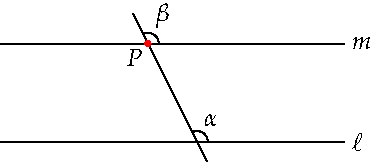
\includegraphics{history-playfair}
\end{minipage}

\begin{itemize}
  \item[]This is equivalent to the existence of a parallel $m$ to a given line $\ell$ through a point $P\not\in\ell$.
\end{itemize}

\boldinline{Arguments requiring unique parallels}\phantomsection\label{pg:absolute}

The following results were proved using Playfair's axiom or the parallel postulate: the \emph{arguments} are therefore false in absolute geometry.
\begin{itemize}
  \item A line crossing parallel lines makes equal angles: in the picture,  $\ell\parallel m\implies \alpha\cong\beta$. This is the uniqueness claim in Playfair: the parallel $m$ to $\ell$ through $P$ is unique.
  \item Angles in a triangle sum to a \ang{180}.
  \item Constructions of squares/rectangles.
  \item Pythagoras' Theorem.
\end{itemize}

While our \emph{arguments} for the above are false in absolute geometry, we cannot instantly claim that the \emph{results} are false; there might be alternative proofs! To show that the results require unique parallels, we must exhibit a \emph{model} in which they are false; such will be described in the next section. The existence of this model explains why Saccheri and Lambert failed in their endeavors: the parallel postulate (Playfair) is indeed independent of Euclid's (Hilbert's) other axioms.
\goodbreak



\begin{minipage}[t]{0.62\linewidth}\vspace{0pt}
\boldsubsubsection{The Saccheri--Legendre Theorem}

We work in absolute geometry, starting with an extension of the exterior angle theorem based on Euclid's proof.\smallbreak
Suppose $\triangle ABC$ has angle sum $\Sigma_\triangle$ and construct $M$ and $E$ following Euclid to obtain congruent triangles as in the picture. Observe:
\end{minipage}\hfill\begin{minipage}[t]{0.36\linewidth}\vspace{0pt}
\flushright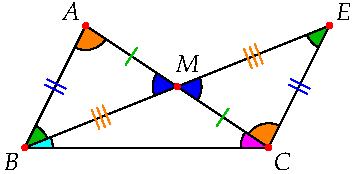
\includegraphics{history-saccheri}
\end{minipage}

\begin{enumerate}\def\lgbullet#1{\raisebox{-3pt}{\textcolor{#1}{\LARGE\textbullet}}}
  \item $\textcolor{magenta}{\measuredangle ACB}+\textcolor{orange}{\measuredangle CAB}=\textcolor{magenta}{\measuredangle ACB}+\textcolor{orange}{\measuredangle ACE}<\ang{180}$ is the exterior angle theorem. More generally, the exterior angle theorem says that the sum of \emph{any two} angles in a triangle is less than \ang{180}.
  \item $\triangle ABC$ and $\triangle EBC$ have the \emph{same angle sum}
  \[\Sigma_\triangle=\lgbullet{orange}+\lgbullet{Green} +\lgbullet{Cyan} +\lgbullet{magenta}\]
  This follows from the picture; remember that we do not know whether $\Sigma_\triangle=\ang{180}$! %remember that \footnote{With the parallel postulate, we could use congruence of angles $\angle BAC\cong\angle ECA$ to conclude that $\cl{CE}\parallel\cl{BA}$, from which the sum of the angles in a triangle is \ang{180} and the observation is trivial. We cannot do this in absolute geometry!}
  \item $\triangle EBC$ has at least one angle ($\textcolor{cyan}{\measuredangle EBC}$ or $\textcolor{Green}{\measuredangle BEC}$) measuring $\le\frac 12\measuredangle ABC$.
\end{enumerate}
Iterate this construction to produce a sequence $\triangle_0=\triangle ABC$, $\triangle_1=\triangle EBC$, $\triangle_2$, $\triangle_3,\ldots$ each of which has the same angle sum $\Sigma_\triangle$ \emph{and} such that at least one angle in $\triangle_n$ has measure
\[\alpha_n\le\frac 1{2^n}\measuredangle ABC\]
Now suppose $\Sigma_\triangle=\ang{180}+\epsilon$ is \emph{greater} than \ang{180}. Since $\frac 1{2^n}\to 0$, we may choose $n$ large enough that $\alpha_n<\epsilon$. But then the sum of the \emph{other two} angles in $\triangle_n$ would be \emph{greater than \ang{180}}, contradicting the exterior angle theorem! In conclusion:

\begin{thm}{Saccheri--Legendre}{saccleg}
In absolute geometry, triangles have angle sum $\Sigma_\triangle\le \ang{180}$.
\end{thm}

Saccheri's failed hope was to prove \emph{equality} without invoking the parallel postulate. That he got half way is still remarkable!

\boldinline{Saccheri and Lambert Quadrilaterals}

Saccheri and Lambert both considered \emph{quadrilaterals} in absolute geometry. Two families of such are named in their honor.

\begin{defn}[lower separated=false, sidebyside, sidebyside align=top seam, sidebyside gap=0pt, righthand width=0.34\linewidth]{}{}
A \emph{Saccheri quadrilateral} $ABCD$ satisfies
\[\cl{AD}\cong\cl{BC}\quad\text{and}\quad \measuredangle DAB=\measuredangle CBA=\ang{90}\]
$\cl{AB}$ is the \emph{base} and $\cl{CD}$ the \emph{summit.}\smallbreak
The interior angles at $C$ and $D$ are the \emph{summit angles.}\medbreak
A \emph{Lambert quadrilateral} has three right-angles; for instance $AMND$  in the picture.
\tcblower
\flushright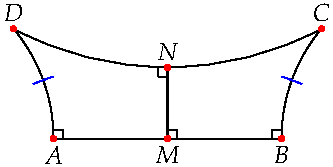
\includegraphics{history-quad3}
\end{defn}

We draw these with curved sides to indicate that the summit angles need not be right-angles, though we haven't yet exhibited a model which shows that they could be anything else. Regardless of how they are drawn, $\cl{AD}$, $\cl{BC}$ and $\cl{CD}$ are all \emph{segments}!
\goodbreak

The seeming symmetry of a Saccheri quadrilateral is not an illusion.

\begin{lemm}[lower separated=false, sidebyside, sidebyside align=top seam, sidebyside gap=0pt, righthand width=0.34\linewidth]{}{saccheribasic}
\exstart If the base and summit of a Saccheri quadrilateral are bisected, we obtain congruent Lambert quadrilaterals.
\begin{enumerate}\setcounter{enumi}{1}
  \item The summit angles of a Saccheri quadrilateral are congruent.
	\item In Euclidean geometry, Saccheri and Lambert quadrilaterals are rectangles (four right-angles).
\end{enumerate}
\tcblower
\flushright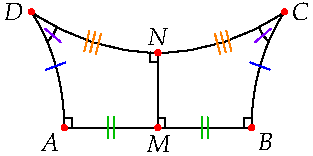
\includegraphics{history-quad4}
\end{lemm}

We leave parts 1 and 2 as an exercise.

\begin{proof}[Proof of 3.]
By part 1 we need only prove this for a Saccheri quadrilateral.
Following the exterior angle theorem, $\overleftrightarrow{AB}$ is a crossing line making equal (right-) angles, whence $\cl{AD}\parallel\cl{BC}$.\\[4pt]
However $\overleftrightarrow{CD}$ also crosses the same parallel lines; by the parallel postulate, the summit angles sum to a straight edge. Since these are congruent, they must both be right-angles. 
\end{proof}

We can now prove another of the conclusions of Saccheri \& Lambert, which justifies our drawing of \emph{acute} summit angles.

\begin{thm}{}{summit90}
The summit angles of a Saccheri quadrilateral measure $\le \ang{90}$. 
\end{thm}

\begin{tcolorbox}[proofstyle, lower separated=false, sidebyside, sidebyside align=top seam, sidebyside gap=0pt, righthand width=0.34\linewidth]
\emph{Proof.} \ Extend $\cl{CB}$ to $E$ (on the opposite side of $\cl{AB}$ to $C$) such that $\cl{BE}\cong\cl{DA}$. Let $M$ be the midpoint of $\cl{AB}$.\smallbreak
SAS implies $\angle AMD\cong \triangle BME$, whence $M$ lies on $\cl{DE}$.\smallbreak
The (congruent) summit angles at $C$ and $D$ therefore sum to
\begin{align*}
\measuredangle ADC+\measuredangle BCD&=\measuredangle ADM+\measuredangle EDC+\measuredangle DCE\\
&=\measuredangle CED+\measuredangle EDC+\measuredangle DCE \le \ang{180}
\end{align*}
by the Saccheri--Legendre Theorem.
\tcblower
\flushright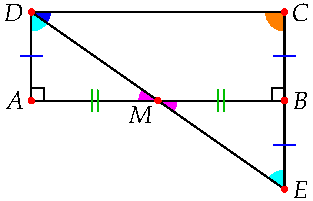
\includegraphics[scale=0.9]{history-quad2}\\[10pt]
\hfill\qedsymbol
\end{tcolorbox}





\begin{exercises}
Complete these exercises in absolute geometry; you cannot use Playfair's Axiom or Euclid's parallel postulate!

\begin{minipage}[t]{0.64\linewidth}\vspace{-5pt}
\begin{enumerate}
  \item Prove parts 1 and 2 of Lemma \ref{lemm:saccheribasic}.\par
  (\emph{Hint: use the picture: all you need are the triangle congruence theorems!})
	\item Use the same picture to give a quick alternative proof of Theorem \ref{thm:summit90}.

	\item\label{exs:rectanglesplit} Suppose $\square ABCD$ has four right-angles. Show that $\cl{AC}$ splits $\square ABCD$ into two congruent triangles, and conclude that the opposite sides are congruent.\par
	Why is this question \emph{much} easier in Euclidean geometry?
\end{enumerate}
\end{minipage}\begin{minipage}[t]{0.35\linewidth}\vspace{-15pt}
\flushright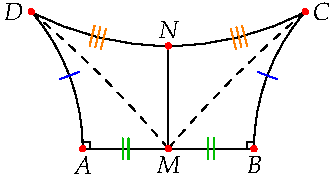
\includegraphics[scale=1]{history-saccheri2}\\
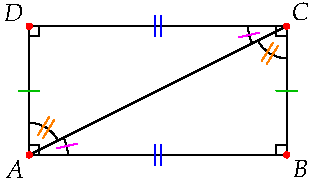
\includegraphics{basic-rect}
\end{minipage}
\end{exercises}

\clearpage



\subsection{Models of Hyperbolic Geometry}\label{sec:hyp-models}

In the early 1800s, James Boylai, Carl Friedrich Gauss and Nikolai Lobashevsky independently took the next step. Rather than attempting to establish the parallel postulate as a theorem within Euclidean geometry, they defined a new geometry based on the first four of Euclid's postulates plus an alternative to the parallel postulate:

\begin{axiom}{Boylai--Lobashevshky/Hyperbolic Postulate}{}
Given a line $\ell$ and a point $P\not\in\ell$, there exist \emph{at least two} parallel lines to $\ell$ through $P$.
\end{axiom}

The resulting axiomatic system\footnote{Formally, we assume all of Hilbert's axioms, replacing Playfair axiom with the hyperbolic postulate.} is called \emph{hyperbolic geometry.} Consistency was proved in the late 1800s by Beltrami, Klein and Poincaré, each of whom created models by defining point, line, etc., in novel ways. One of the simplest is named for Poincaré, though was first proposed by Beltrami.

\begin{defn}[lower separated=false, sidebyside, sidebyside align=top seam, sidebyside gap=0pt, righthand width=0.3\linewidth]{}{poincaredisk}
The \emph{Poincaré disk} is the interior of the unit circle
	\[\bigl\{(x,y):x^2+y^2<1\bigr\}\]
A \emph{hyperbolic line} is a diameter or a circular arc meeting the unit circle at right-angles.\smallbreak
In the picture we have a \textcolor{red}{hyperbolic line $\ell$} and a \textcolor{blue}{point $P$}: also drawn are several \textcolor{Green}{parallel hyperbolic lines} to $\ell$ passing through $P$.\smallbreak
Points on the boundary circle are termed \emph{omega-points}: these are \emph{not} in the Poincaré disk and are essentially `points at infinity.' 
\tcblower
\flushright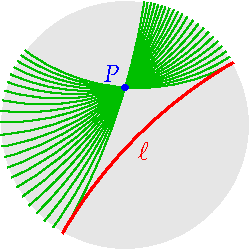
\includegraphics{models-parallels}
\end{defn}

Since it depends only on the incidence axioms, there exists a unique hyperbolic line joining any two points in the Poincaré disk.\par

Hyperbolic lines may straightforwardly be described using equations in analytic geometry.

\begin{lemm}[lower separated=false, sidebyside, sidebyside align=top seam, sidebyside gap=0pt, righthand width=0.35\linewidth]{}{hypline}
Every hyperbolic line in the Poincaré disk model is one of the following:
\begin{itemize}
  \item A diameter passing through $(c,d)\neq (0,0)$ with Euclidean equation $dx=cy$.
  \item The arc of a (Euclidean) circle with equation
	\[x^2+y^2-2ax-2by+1=0\quad\text{where}\quad a^2+b^2>1\]
	and (Euclidean) center and radius
	\[C=(a,b)\quad\text{and}\quad r=\sqrt{a^2+b^2-1}\]
\end{itemize}
\tcblower
\flushright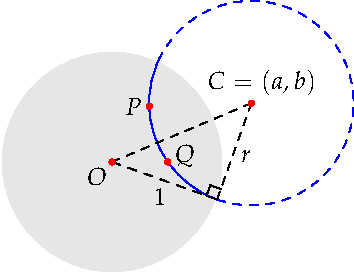
\includegraphics[scale=0.9]{models-example}
\end{lemm}\goodbreak

\begin{example}{}{}
We compute the hyperbolic line through $P=(0,\frac 12)$ and $Q=(\frac 12,\frac 13)$ in the Poincaré disk: this is the picture shown in Lemma \ref{lemm:hypline}.\smallbreak
Substitute into $x^2+y^2-2ax-2by+1=0$ to obtain a system of equations for $a,b$:
\[\begin{cases}
\frac 14-b+1=0\\
\frac 14+\frac 19-a-\frac 23b+1=0
\end{cases}\implies (a,b)=\left(\frac{19}{36},\frac 54\right)\]
The required hyperbolic line $\lin{PQ}$ therefore has equation
\[x^2+y^2-\frac{19}{18}x-\frac{5}{2}y+1=0\quad\text{or}\quad \left(x-\frac{19}{36}\right)^2+\left(y-\frac 54\right)^2=\frac{545}{648}\]
\end{example}

\emph{On} and \emph{between} now make sense. To complete the model, we need to define congruence of hyperbolic segments and angles.

\begin{defn*}{\ref{defn:poincaredisk} continued}
The \emph{hyperbolic distance} between points $P,Q$ in the Poincaré disk is

\begin{minipage}[t]{0.7\linewidth}\vspace{-12pt}
	\[d(P,Q):=\cosh^{-1}\left(1+\frac{2\nm{PQ}^2}{(1-\nm{P}^2)(1-\nm{Q}^2)}\right)\]
	where $\nm{PQ}$ is the Euclidean distance and $\nm P,\nm Q$ are the Euclidean distances of $P,Q$ from the origin.\smallbreak
	Hyperbolic line segments are \emph{congruent} if they have the same length.\smallbreak
	The \emph{angle} between hyperbolic rays is that between their (Euclidean) tangent lines: angles are congruent if they have the same measure.
	\end{minipage}\begin{minipage}[t]{0.3\linewidth}\vspace{-5pt}
	\flushright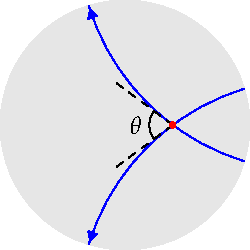
\includegraphics{models-angle}
	\end{minipage}
\end{defn*}

\begin{lemm}{}{distformula}
The hyperbolic distance\footnotemark{} of $P$ from the origin is
\[d(O,P)=\cosh^{-1}\frac{1+\nm P^2}{1-\nm P^2}=\ln\frac{1+\nm P}{1-\nm P}\]
\end{lemm}

\footnotetext{It seems reasonable for hyperbolic functions to play some role in hyperbolic geometry! As a primer:
  \[\cosh x=\frac{e^x+e^{-x}}2,\quad \sinh x=\frac{e^x-e^{-x}}2,\quad\tanh x=\frac{\sinh x}{\cosh x}=\frac{e^x-e^{-x}}{e^x+e^{-x}}\quad\text{and}\quad\cosh^{-1}x=\ln(x+\sqrt{x^2-1})\]\vspace{-15pt}}


\begin{example}{}{hypisosceles}
We calculate the sides and angles in the isosceles right-triangle\par
\begin{minipage}[t]{0.69\linewidth}\vspace{-8pt}
with vertices $O=(0,0)$, $P=(\frac 12,0)$ and $Q=(0,\frac 12)$.
\begin{gather*}
\nm P=\tfrac 12=\nm Q,\qquad \nm{PQ}^2=\tfrac 14+\tfrac 14=\tfrac 12\\
d(O,P)=d(O,Q)=\ln\frac{1+\frac 12}{1-\frac 12}=\ln 3=\cosh^{-1}\frac 53\approx 1.099\\
d(P,Q)=\cosh^{-1}\left(1+\frac{2\cdot \frac 12}{(1-\frac 14)^2}\right) =\cosh^{-1}\frac{25}9 \approx 1.681
\end{gather*}
\end{minipage}\hfill
\begin{minipage}[t]{0.3\linewidth}\vspace{-20pt}
\flushright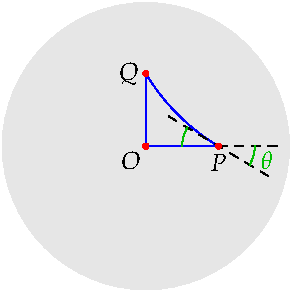
\includegraphics[scale=0.9]{models-dist4}
\end{minipage}
\goodbreak

To find the interior angle $\theta$, implicitly differentiate the equation for the hyperbolic line $\lin{PQ}$:
\[x^2+y^2-\frac 52x-\frac 52y+1=0 \implies \diffat[y]{x}{P}=\frac{4x-5}{5-4y}\bigg|_P=-\frac 35 \implies \theta=\tan^{-1}\frac 35\approx \ang{30.96}\]
By symmetry, we have the same angle at $Q$. With a right-angle at $O$, we conclude that the angle sum is approximately $\Sigma_\triangle=\ang{151.93}$!\smallbreak
As a sanity check, we compare data for $\triangle OPQ$ and the \emph{Euclidean} triangle with the same vertices
\begin{center}
\begin{tabular}{l||c|c}
Property&Hyperbolic Triangle&Euclidean Triangle\\\hline\hline
Edge lengths&$1.099:1.099:1.681$&$0.5:0.5:0.707$\\
Relative edge ratios&$1:1:1.530$&$1:1:1.414$\\
Angles&\ang{30.06}, \ang{30.96}, \ang{90}&\ang{45}, \ang{45}, \ang{90}%\\
%Area&1.023&0.322
\end{tabular}
\end{center}
The hyperbolic triangle has longer sides and a \emph{relatively} longer hypotenuse. Moreover, its side lengths do \emph{not} satisfy the Pythagorean relation $a^2+b^2=c^2$ (we'll revisit this in Theorem \ref{thm:hyptrig}).
\end{example}

\begin{minipage}[t]{0.65\linewidth}\vspace{-5pt}
The next result is an exercise; it says that distance increases smoothly as one moves along a hyperbolic line.

\begin{lemm}{}{hypdistwd}
Fix $P$ and a hyperbolic line through $P$. Then the distance function $Q\mapsto d(P,Q)$ maps the set of points on one side of $P$ differentiably and bijectively onto the interval $(0,\infty)$.
\end{lemm}

The Lemma means that hyperbolic circles are well-defined and look like one expects: the circle of hyperbolic radius $\delta$ centered at $P$ is the set of points $Q$ such that $d(P,Q)=\delta$.
\end{minipage}\hfill\begin{minipage}[t]{0.35\linewidth}\vspace{-5pt}
\flushright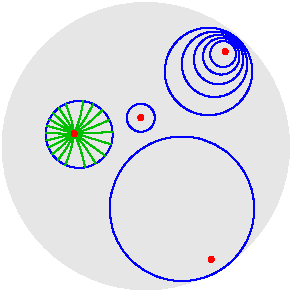
\includegraphics[scale=0.95]{hyper-circle}
\end{minipage}\medbreak

In the picture are several \textcolor{blue}{hyperbolic circles} and their \textcolor{red}{centers}; one has several of its \textcolor{Green}{radii} drawn. Observe how the centers are closer (in a Euclidean sense) to the boundary circle than one might expect: this is since hyperbolic distances measure greater the further one is from the origin.\smallbreak

In fact (Exercise \ref*{sec:hyp-models}.\ref{exs:circhypcirc}) hyperbolic circles in the Poincaré disk model are also Euclidean circles! Their hyperbolic radii moreover intersect the circles at right-angles, as we'd expect.


\begin{thm}{}{}
The Poincaré disk is a model of hyperbolic geometry.
\end{thm}

\begin{proof}[Sketch Proof]
A rigorous proof would require that we check the hyperbolic postulate and all Hilbert's axioms except Playfair. Instead we check Euclid's postulates 1--4 and the hyperbolic postulate 5.
\begin{enumerate}\itemsep0pt
  \item Lemma \ref{lemm:hypline} says we can join any given points in the Poincaré disk by a unique segment.
  \item A hyperbolic segment joins two points \emph{inside} the (open) Poincaré disk. The distance formula increases (Lemma \ref{lemm:hypdistwd}) unboundedly as $P$ moves towards the boundary circle, so we can always make a hyperbolic line longer.
  \item Hyperbolic circles are defined above.
  \item All right-angles are equal since the notion of angle is unchanged from Euclidean geometry.
  \item The first picture on page \pageref{sec:hyp-models} shows multiple parallels!\hfill{\qedhere}
\end{enumerate}
\end{proof}

\goodbreak



\boldsubsubsection{Other Models of Hyperbolic Space: non-examinable}

There are several other models of hyperbolic space. Here are three of the most common.%\vspace{-8pt}

\boldinline{Klein Disk Model} This is similar to the Poincaré disk, though lines are chords of the unit circle (`Euclidean' straight lines!) and the distance function is different:
\[d_K(P,Q)=\frac 12\nm{\ln\frac{\nm{P\Theta}\nm{Q\Omega}}{\nm{P\Omega}\nm{Q\Theta}}}\]

\begin{minipage}[t]{0.69\linewidth}\vspace{0pt}
where $\Omega,\Theta$ are where the chord $\smash[t]{\lin{PQ}}$ meets the boundary circle.\smallbreak
The cost is that the notion of \emph{angle} is different. The picture shows perpendicularity: Given a \textcolor{red}{hyperbolic line} find the \textcolor{Green}{tangents} to where it meets the boundary circle. Any \textcolor{blue}{chord} whose extension passes through the \textcolor{Green}{intersection} of these tangents is perpendicular to the \textcolor{red}{original line}. Measuring other angles is difficult!
\end{minipage}
\begin{minipage}[t]{0.3\linewidth}\vspace{-32pt}
\flushright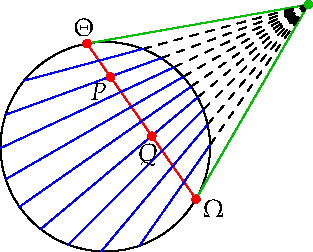
\includegraphics[scale=0.9]{models-klein}
\end{minipage}\medbreak

Gauss' famous theorem egregium says that this problem is unavoidable; there is no model in which lines and angles both have the same meaning as in Euclidean geometry. 

%  If $H$ is a model of hyperbolic geometry, then its intrinsic curvature says that it is impossible to find an embedding $f:H\to\R^2$ which preserves \emph{both} the concepts of straight line and angle. Poincaré's model has nice angles but `bendy' lines; Klein's lines are `Euclidean straight' but his angle are ugly. The best we can do is to have one concept or the other: we cannot have both.\footnote{The same problem arises when trying to make a map of part of the Earth (another curved geometry). One can have maps which preserve distance or angle, but not both.}

\begin{minipage}[t]{0.69\linewidth}\vspace{0pt}
\boldinline{Poincaré Half-plane Model}

Widely used in complex analysis, the points comprise the upper half-plane $(y>0)$ in $\R^2$, while hyperbolic lines are verticals or semicircles centered on the $x$-axis
\[x=\text{constant}\quad\text{or}\quad (x-a)^2+y^2=r^2\]
and angles are the same as in Euclidean space. The expression for hyperbolic distance remains horrific! The picture shows several hyperbolic lines and a \textcolor{blue}{hyperbolic triangle.}
\end{minipage}\hfill\begin{minipage}[t]{0.3\linewidth}\vspace{0pt}
	\flushright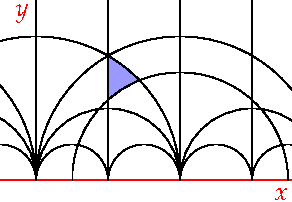
\includegraphics{models-halfplane}
\end{minipage}



\boldinline{Hyperboloid Model}

Points comprise the upper sheet $(z\ge 1)$ of the hyperboloid $x^2+y^2=z^2-1$. A \textcolor{blue}{hyperbolic line} is the intersection of the hyperboloid with a plane through the origin. Isometries (congruence) can be described using matrix-multiplication and hyperbolic distance is relatively easy: given $P=(x,y,z)$ and $Q=(a,b,c)$, hyperbolic distance is

\begin{minipage}[t]{0.6\linewidth}\vspace{-10pt}
\begin{gather*}
d(P,Q)=\cosh^{-1}(cz-ax-by)
\end{gather*}
Difficulties include working in three dimensions and the fact that angles are awkward.\smallbreak
The relationship to the Poincaré disk is via projection. Place the disk in the $x,y$-plane centered at the origin and draw a \textcolor{Green}{line} through the disk and the point $(0,0,-1)$. The intersection of this line with the hyperboloid gives the correspondence.
\end{minipage}\begin{minipage}[t]{0.4\linewidth}\vspace{0pt}
\flushright\href{http://www.math.uci.edu/~ndonalds/math161/hyper-plane.html}{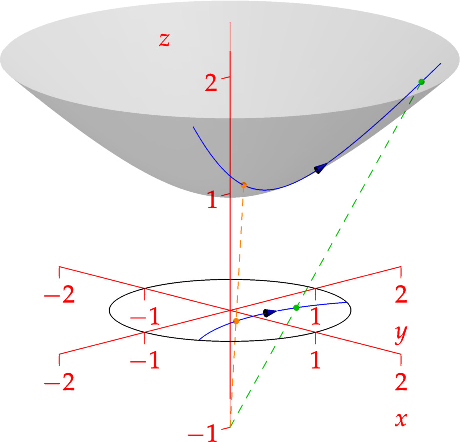
\includegraphics[scale=0.8]{hyper-plane}}
\end{minipage}

\begin{exercises}
All questions are  within the Poincaré disk model
\begin{enumerate}
  \item\begin{enumerate}
    \item Find the equation of the hyperbolic line joining $P=(\frac 14,0)$ and $Q=(0,\frac 12)$.
    \item Find the side lengths of the hyperbolic triangle $\triangle OPQ$ where $O=(0,0)$ is the origin.
    \item The triangle in part (b) is right-angled at $O$. If $o,p,q$ represent the hyperbolic lengths of the sides opposite $O,P,Q$ respectively, check that the Pythagorean theorem $p^2+q^2=o^2$ is \emph{false.} Now compute $\cosh p\cosh q$: what do you observe?
  \end{enumerate}
  	
  \item Let $P=\left(\frac 12,\sqrt{\frac 5{12}}\right)$ and $Q=\left(\frac 12,-\sqrt{\frac 5{12}}\right)$
  \begin{enumerate}
    \item Compute the hyperbolic distances $d(O,P)$, $d(O,Q)$ and $d(P,Q)$, where $O$ is the origin.
    \item Compute the angle $\measuredangle POQ$.
	  \item Show that the hyperbolic line $\ell=\lin{PQ}$ has equation
		\[x^2-\frac{10}3x+y^2+1=0\]
  	\item Calculate $\diff[y]{x}$ and hence show that a tangent vector to $\ell$ at $P$ is $\sqrt{15}\vi+7\vj$. Use this to compute $\measuredangle OPQ$.
	\end{enumerate} 
	
  \item\label{exs:isorighthypextended} We extend Example \ref{ex:hypisosceles}. Let $c\in(0,1)$ and label $O=(0,0)$, $P=(c,0)$ and $Q=(0,c)$.
  \begin{enumerate}
    \item Compute the hyperbolic side lengths of $\triangle OPQ$.
    \item Find the equation of the hyperbolic line joining $P=(c,0)$ and $Q=(0,c)$.
    \item Use implicit differentiation to prove that the interior angles at $P$ and $Q$ measure $\tan^{-1}\frac{1-c^2}{1+c^2}$. What happens as $c\to 0^+$ and as $c\to 1^-$?
  \end{enumerate}
	
	\item Let $0<r<1$ and find the hyperbolic side lengths and interior angles of the equilateral triangle with vertices $(r,0)$, $(-\frac r2,\frac{\sqrt 3r}2)$ and $(-\frac r2,-\frac{\sqrt 3r}2)$.What do you observe as $r\to 0^+$ and $r\to 1^-$?
	
	\item\label{exs:circhypcirc}\begin{enumerate}
    \item Use the cosh distance formula to prove that the hyperbolic circle of hyperbolic radius $\rho=\ln 3$ and center $C=(\frac 12,0)$ in the Poincaré disk has \emph{Euclidean} equation
    \[\left(x-\frac 25\right)^2+y^2=\frac 4{25}\]
    \item Prove that every hyperbolic circle in the Poincaré disk is in fact a Euclidean circle.
  \end{enumerate}
	
	\item We sketch a proof of Lemma \ref{lemm:hypdistwd}. 
	\begin{enumerate}
	  \item Prove that $f(x)=\cosh^{-1}x=\ln(x+\sqrt{x^2-1})$ is strictly increasing on the interval $(1,\infty)$.
	  \item By part (a), it is enough to show that $\frac{\nm{PQ}^2}{1-\nm Q^2}$ increases as $Q$ moves away from $P$ along a hyperbolic line. Appealing to symmetry, let $P=(0,c)$ lie on the hyperbolic line with equation $x^2+y^2-2by+1=0$. Prove that
	  \[\frac{\nm{PQ}^2}{1-\nm Q^2}=\frac{(b-c)y+bc-1}{1-by}\]
	  and hence show that this is an increasing function of $y$ when $c<y<\frac 1b$.
	\end{enumerate} 
% For a difficult exercise, try to find the omega-points for the line $\overleftrightarrow{PQ}$ and see that you obtain the same expression for the distance.\footnote{Hint: $\Omega,\Theta$ have $x=\frac{4\pm\sqrt{34}}{10}$, $y=\frac{4\mp\sqrt{34}}{10}$\ldots}\goodbreak


\end{enumerate}
\end{exercises}

\clearpage


\subsection{Parallels, Perpendiculars \& Angle-Sums}\label{sec:hypparallel}

\begin{minipage}[t]{0.65\linewidth}\vspace{-8pt}
From now on, all examples will be illustrated within the Poincaré disk model. Recall (page \pageref{sec:hyp1}) that we may use anything from absolute geometry; as a sanity check, think through how the picture illustrates the following result.

\begin{lemm}{}{hypperp}
Through a point $P$ not on a line $\ell$ there exists a unique perpendicular to $\ell$. 
\end{lemm}

%\medskip

We now consider a major departure from Euclidean geometry.
\end{minipage}\hfill\begin{minipage}[t]{0.34\linewidth}\vspace{-28pt}
\flushright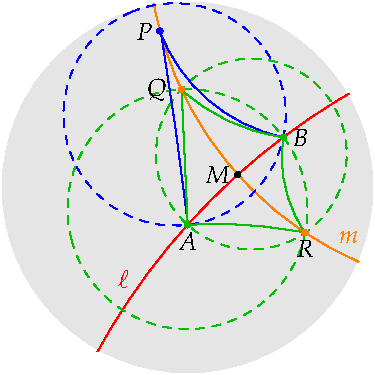
\includegraphics[scale=0.75]{basic-perp}
\end{minipage}

% \begin{proof}
% Choose a point $A\in\ell$ and join $\cl{AP}$. If $\cl{AP}$ is perpendicular to $\ell$, we only need uniqueness.\par
% \begin{minipage}[t]{0.63\linewidth}\vspace{-3pt}
% Otherwise, $\ell$ is \emph{not tangent} to the \textcolor{blue}{circle} centered at $P$ with radius $\nm{AP}$. There therefore exists a second intersection point $B\in\ell$.\smallbreak
% Construct the \textcolor{Green}{circles} with radius $\nm{AB}$ centered at $A$ and $B$ respectively: these have two intersections $Q,R$. Let $\textcolor{orange}{m}=\lin{QR}$.\smallbreak
% Fhe following should be straightforward:
% \begin{itemize}\itemsep0pt
%   \item $m$ intersects $\ell$ at right-angles ($M$ in the picture)
%   \item $P\in m$
%   \item $M$ is the midpoint of $\cl{AB}$
% \end{itemize}
% To help, note that the blue and green arcs are radii of their respective circles, so we have several isosceles triangles\ldots 
% \end{minipage}\hfill\begin{minipage}[t]{0.36\linewidth}\vspace{0pt}
% \flushright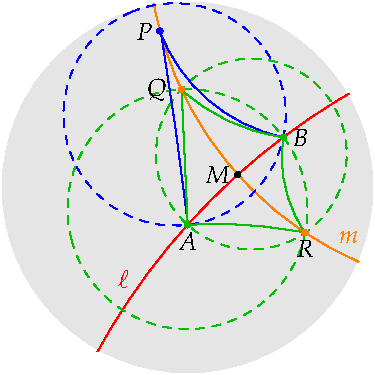
\includegraphics[scale=0.9]{basic-perp}
% \end{minipage}\smallbreak
% For uniqueness, suppose we have two perpendiculars to $\ell$ through $P$ intersecting $\ell$ at distinct points $M,N$. Then $\triangle PMN$ has two right-angles which contradicts Saccheri--Legendre (Theorem \ref{thm:saccleg}).
% \end{proof}



%\boldsubsubsection{The Fundamental Theorem of Parallels in Hyperbolic Geometry}


\begin{thm}[lower separated=false, sidebyside, sidebyside align=top seam, sidebyside gap=0pt, righthand width=0.25\linewidth]{Fundamental Theorem of Parallels}{hyperfund}
Given $P\not\in\textcolor{red}{\ell}$, drop the perpendicular $\cl{PQ}$. Then there exist precisely two \textcolor{blue}{parallel lines $m,n$} to $\ell$ through $P$ with the following properties:
\begin{enumerate}\itemsep0pt
  \item A \textcolor{Green}{ray} based at $P$ intersects $\ell$ if and only if it lies between $m$ and $n$ in the same fashion as $\ray{PQ}$.
  \item $m$ and $n$ make congruent acute angles $\mu$ with $\ray{PQ}$.
\end{enumerate}
\tcblower
\flushright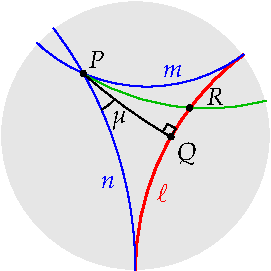
\includegraphics[scale=0.8]{basic-parallels}
\end{thm}

\begin{defn}{}{limparallel}
The lines $m,n$ are the \emph{limiting,} or \emph{asymptotic, parallels} to $\ell$ through $P$. Every other parallel is termed \emph{ultraparallel.} The \emph{angle of parallelism} at $P$ relative to $\ell$ is the acute angle $\mu$.
\end{defn}

More generally, parallel lines $\ell,m$ are \emph{limiting} if the `meet' at an omega-point.\smallbreak


The proof depends crucially on ideas from analysis, particularly continuity \& suprema.
 
\begin{proof}
Points $R\in\ell$ are in continuous bijective correspondence with the real numbers (Lemma \ref{lemm:hypdistwd}). It follows that we have a \emph{continuous} function
\[f:\R\to(-\ang{90},\ang{90}]\quad\text{where}\quad f(r)=\measuredangle QPR\]
By the exterior angle theorem, $\ang{90}\not\in\operatorname{range}f$. Since $\dom f=\R$ is an interval, the intermediate value theorem forces $\operatorname{range}f$ to be a \emph{subinterval} $I\subseteq(-\ang{90},\ang{90})$.\smallbreak
Transfer $\cl{QR}$ to the other side of $Q$ to produce $S\in\ell$. Applying SAS we see that $\measuredangle QPS=-\measuredangle QPR$, whence the interval $I=\operatorname{range}f$ is \emph{symmetric}:
\[\theta\in I\iff -\theta\in I\]
Define $\mu:=\sup I\le\ang{90}$ to be the least upper bound; by symmetry, $-\mu=\inf I$. Let $m$ and $n$ be the lines making angles $\pm\mu$ respectively. Plainly every ray making angle $\theta\in(-\mu,\mu)$ intersects $\ell$.\smallbreak
Suppose $m$ intersected $\ell$ at $M$. Let $\tilde M\in\ell$ lie on the other side of $M$ from $Q$. Then $\measuredangle QP\tilde M>\mu$ contradicts $\mu=\sup I$. It follows that $m$ is parallel to $\ell$. Similarly $n\parallel\ell$ and we have part 1.\smallbreak
Finally $m=n\iff \mu=\ang{90}$. In such a case there would exist only one parallel to $\ell$ through $P$, contradicting the hyperbolic postulate.
\end{proof}

Except for the last line, the proof is valid in Euclidean geometry, where $I=(-\ang{90},\ang{90})$ and $\mu=\ang{90}$!\medbreak\goodbreak


The picture suggests a tight relationship between $\mu$ and the perpendicular distance. Here it is, though we postpone the proof to Exercise \ref*{sec:hypparallel}.\ref{exs:angparallelism}.% and a discussion of omega-triangles.

%\smallbreak
% In Exercise \hyperref[exs:angparallelism]{\ref*{sec:hypparallel}.\ref*{exs:angparallelism}} we show that the perpendicular (hyperbolic) distance $\delta=\nm{PQ}$ is bijectively related to the angle of parallelism:
% \[\cosh\delta=\csc\mu\quad\text{or equivalently}\quad \tan\frac{\mu}2=e^{-\delta}\tag{$\ast$}\]
\goodbreak
\begin{cor}{}{parangleformula}
The perpendicular distance $\delta=d(P,Q)$ and the angle of parallelism are related via
\[\cosh\delta=\csc\mu\quad\text{or equivalently}\quad \tan\frac{\mu}2=e^{-\delta}\]
\end{cor}


% \begin{minipage}[t]{0.7\linewidth}\vspace{0pt}
% \boldinline{Example}
% 
% Find the limiting parallels and the angle of parallelism for the point $P=(-\frac 3{10},\frac 4{10})$ and the \textcolor{red}{hyperbolic line} with equation $x^2+y^2+2x+3y+1=0$.\\[5pt]
% First find the omega-points by intersecting with the boundary circle $x^2+y^2=1$:
% \[\Omega=(-1,0),\quad \Theta=\left(\frac 5{13},-\frac{12}{13}\right)\]
% $P$ does not lie on a diameter containing $\Omega$ or $\Theta$, whence we substitute these points into the usual expression $x^2+y^2-2ax-2by+1=0$ for a hyperbolic line and solve for $(a,b)$ in each case. We obtain
% \end{minipage}\begin{minipage}[t]{0.3\linewidth}\vspace{0pt}
% \flushright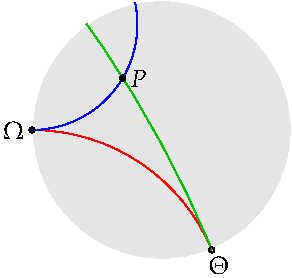
\includegraphics{basic-parallels2}
% \end{minipage}\\[10pt]
% \begin{itemize}
%   \item[] \textcolor{blue}{$\overleftrightarrow{P\Omega}$}:\quad $x^2+y^2+2x-\frac{13}8y+1=0$ with center $(a,b)=(-1,\frac{13}{16})$
%   \item[] \textcolor{Green}{$\overleftrightarrow{P\Theta}$}:\quad $x^2+y^2+\frac{127}8x+\frac{281}{32}y+1=0$\quad with center $(a,b)=(-\frac{127}{16},-\frac{281}{64})$
% \end{itemize}

\begin{examples}{}{}
\exstart Let $\textcolor{red}{\ell}$ be the hyperbolic line $x^2+y^2-4x+1=0$.\par
\begin{enumerate}\setcounter{enumi}{1}
\begin{minipage}[t]{0.7\linewidth}\vspace{-5pt}
  \item[]Intersect with $x^2+y^2=1$ to find $\Omega=\left(\tfrac 12,\tfrac{\sqrt 3}2\right)$ and $\Theta=\left(\tfrac 12,-\tfrac{\sqrt 3}2\right)$.\par
	By symmetry, the perpendicular from $P=(0,0)$ to $\ell$ has equation $y=0$ and results in $Q=(2-\sqrt 3,0)$. \smallbreak
	The limiting parallels through $P$ have equations $y=\pm\sqrt 3x$, from which the angle of parallelism is $\mu=\tan^{-1}\sqrt 3=\ang{60}$.\par
  In accordance with Corollary \ref{cor:parangleformula}, we easily verify that
\end{minipage}\begin{minipage}[t]{0.3\linewidth}\vspace{-25pt}
  \flushright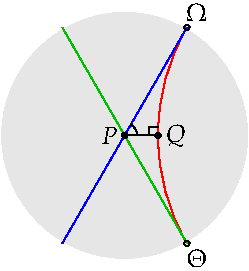
\includegraphics{basic-parallels4}
\end{minipage}\par\vspace{-15pt}
	\[\delta=d(P,Q)=\ln\frac{1+(2-\sqrt 3)}{1-(2-\sqrt 3)}=\ln\sqrt 3 \leftrightsquigarrow e^{-\delta}=\frac 1{\sqrt 3}=\tan\frac{\mu}2\]
  
\begin{minipage}[t]{0.68\linewidth}\vspace{0pt}
  \item We find the limiting parallels and the angle of parallelism when
	\[P=\left(-\frac 3{10},\frac 4{10}\right)\quad\text{and}\quad \textcolor{red}{x^2+y^2+2x+4y+1=0}\]
	First find the omega-points by intersecting with $x^2+y^2=1$:
	\[\Omega=(-1,0),\quad \Theta=\left(\frac 35,-\frac 45\right)\]
	Plainly $\textcolor{Green}{\overleftrightarrow{P\Theta}}$ is the diameter $y=-\frac 43x$ with slope $-\frac 43$.
\end{minipage}\begin{minipage}[t]{0.32\linewidth}\vspace{0pt}
	\flushright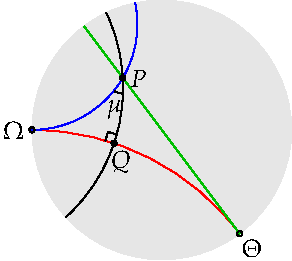
\includegraphics{basic-parallels3}
\end{minipage}\smallbreak
	For $\textcolor{blue}{\overleftrightarrow{P\Omega}}$, substitute into the usual expression $x^2+y^2-2ax-2by+1=0$ and implicitly differentiate:
	\[x^2+y^2+2x-\frac{13}8y+1=0\implies \diffat[y]{x}{P}=\frac{16(1+x)}{13-16y}\bigg|_P=\frac{16\cdot\frac 7{10}}{13-\frac{64}{10}}=\frac{56}{33}\]
	The angle of parallelism is \emph{half} that between the tangent vectors $\stwovec{-33}{-56}$ and $\stwovec 3{-4}$:
\begin{align*}
\mu&=\frac 12\cos^{-1}\frac{\stwovec{-33}{-56}\cdot\stwovec{3}{-4}}{\nm{\stwovec{-33}{-56}}\nm{\stwovec{3}{-4}}}
=\frac 12\cos^{-1}\frac 5{13}\approx \ang{33.69}
\end{align*}
Corollary \ref{cor:parangleformula} can now be used to find the perpendicular distance $d(P,Q)=\ln\frac{3+\sqrt{13}}2$.\par
Without the development of later machinery, it is very tricky to compute $Q$. If you want a serious challenge, see if you can convince yourself that $Q=\left(\frac{93(-29+2\sqrt{117})}{1865},\frac{26(-29+2\sqrt{117})}{1865}\right)$.
\end{enumerate}
\end{examples}

\goodbreak


\boldsubsubsection{Angles in Triangles, Rectangles and the AAA Congruence}

We finish this section three important differences between hyperbolic and Euclidean geometry.

\begin{thm}{}{hyptriangle}
In hyperbolic geometry:
\begin{enumerate}\itemsep0pt
  \item There are no rectangles (quadrilaterals with four right-angles): in particular, the summit angles of a Saccheri quadrilateral are acute.
  \item The angles in a triangle always sum to less than \ang{180}.
  \item (AAA congruence)\lstsp If $\triangle ABC$ and $\triangle DEF$ have angles congruent in pairs, then their sides are congruent in pairs and so $\triangle ABC\cong\triangle DEF$.
\end{enumerate}
\end{thm}

Note that AAA is a triangle \emph{congruence} theorem in hyperbolic geometry, not a \emph{similarity} theorem! Compare with our observations on page \pageref{pg:absolute}. These results largely show that Euclid's arguments requiring the parallel postulate really required it! 







\begin{proof}
Suppose $\square ABCD$ is a rectangle, let $P\in\cl{CD}$ and drop the perpendicular to $R\in\cl{AB}$.\smallbreak
$\square PRBC$ is a rectangle; if not, then one of $\square ARPD$ or $\square PRBC$ would have angle sum exceeding \ang{360}.\smallbreak
By Exercise \ref*{sec:hyp1}.\ref{exs:rectanglesplit}, $\ray{BP}$ splits $\square PRBC$ so that the \textcolor{orange}{marked angles} are congruent. In particular, $\ray{BP}$ crosses $\cl{CD}$ at the \emph{same angle} as it leaves $B$.\smallbreak
Produce a sequence of equidistant points $P_1,P_2,P_3,\ldots$ along $\ray{BP}$, each time dropping the perpendicular back to $\cl{CD}$ to produce the sequence $Q_1,Q_2,Q_3,\ldots$\smallbreak
By SAA, $\triangle PP_1Q_1\cong\triangle BPR$, etc., whence we obtain a second rectangle congruent to $\square PRBC$, etc. In this manner we see that the sequence of points $P,Q_1,Q_2,Q_3,\ldots$ is also \emph{equidistant.} Since $\cl{CD}$ is \emph{finite,} this sequence must eventually pass $D$: we conclude that $\ray{BP}$ intersects $\lin{AD}$.
\begin{center}
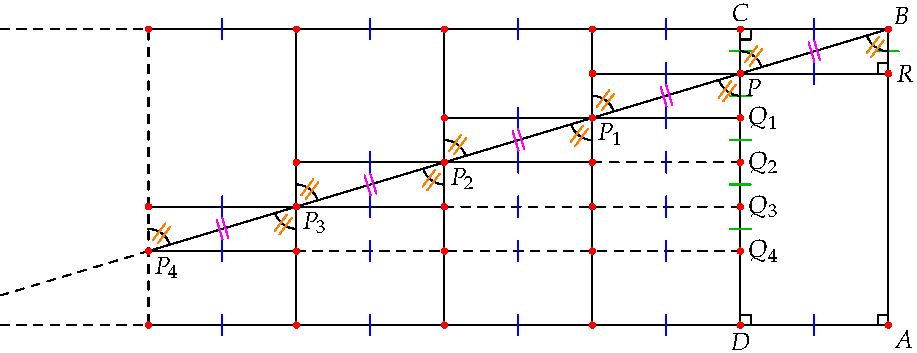
\includegraphics{basic-rect4}
\end{center}
Since $P$ was generic, we see that any ray based at $B$ on the same side as $\cl{AD}$ must intersect $\lin{AD}$. The angle of parallelism of $B$ with respect to $\lin{AD}$ is therefore \ang{90}, whence the hyperbolic postulate is false. There are no rectangles in hyperbolic geometry.\smallbreak
Parts 2 and 3 are corollaries: we address these in the Exercises.
\end{proof}

\goodbreak

\begin{exercises}
\exstart Prove the following in hyperbolic geometry (\emph{use Theorem \ref{thm:hyptriangle}}).\par\vspace{-2pt}
\begin{enumerate}\setcounter{enumi}{1}
  \item[]\begin{enumerate}
    \item Two hyperbolic lines cannot have more than one common perpendicular.
    \item\label{exs:saccherisummitcong} Saccheri quadrilaterals with congruent summits and summit angles are congruent.
  \end{enumerate}
  
  \item Let $\ell$ be the line $x^2+y^2-4x+2y+1=0$ and drop a perpendicular from $O$ to $Q\in\ell$.
  \begin{enumerate}
    \item Explain why $Q$ has co-ordinates $(\frac 2{\sqrt 5}t,-\frac 1{\sqrt 5}t)$ for some $t\in(0,1)$.
    \item Show that the hyperbolic distance $\delta=d(O,Q)$ of $\ell$ from the origin is $\ln\frac{1+\sqrt 5}2$.
    \item By observing that $\Omega=(0,-1)$ is an omega-point for $\ell$, compute the angle of parallelism $\mu=\measuredangle QO\Omega$ explicitly and check that $\cosh\delta=\csc\mu$.
	\end{enumerate}
    
	\item\label{exs:angparallelism} We prove a simplified version of Corollary \ref{cor:parangleformula}.
	Let $P=(0,0)$ be the origin, let $0<r<1$ and consider the hyperbolic line $\ell$ passing through $Q=(r,0)$ at right-angles to $\cl{PQ}$.
  \begin{enumerate}
    \item Find the equation of $\ell$ and prove that the limiting parallels of $\ell$ through $P$ have equations
    \[y=\pm\frac{1-r^2}{2r}x\]
    (\emph{Hint: what does symmetry tell you about the location of the Euclidean center of $\ell$?})
    \item Let $\mu$ be the angle of parallelism of $P$ relative to $\ell$ and $\delta=d(P,Q)$ the hyperbolic distance. Prove that $\cosh\delta=\csc\mu$.\\
    (\emph{Hint: $\csc^2\!\mu=1+\cot^2\!\mu=1+\frac 1{\tan^2\!\mu}=\ldots$})
  \end{enumerate}
  
  \item We work in \emph{absolute geometry}.
  \begin{enumerate}
    \begin{minipage}[t]{0.64\linewidth}\vspace{0pt}
    \item Suppose $A$, $B$ and $P$ are non-collinear and drop the perpendicular from $P$ to $Q\in\overleftrightarrow{AB}$.\par
    If $P$ lies between the perpendiculars $\ell,m$ to $\overleftrightarrow{AB}$ through $A$ and $B$, prove that $Q$ is interior to $\cl{AB}$.\par
    (\emph{Hint: show that the other cases are impossible})
    \item Suppose there exists a triangle with angle sum \ang{180}. Show that there exists a \emph{right-triangle} with angle sum \ang{180} and therefore a rectangle.
  	\end{minipage}\hfill
  	\begin{minipage}[t]{0.35\linewidth}\vspace{0pt}
  		\flushright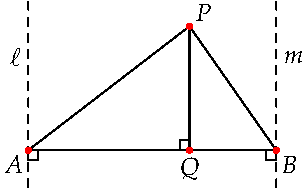
\includegraphics{basic-tri2}
  	\end{minipage}\smallbreak
  	(\emph{Since rectangles are impossible in hyperbolic geometry, this proves part 2 of Theorem \ref{thm:hyptriangle}})
  \end{enumerate}
  
  
  \item We prove the AAA congruence theorem (Theorem \ref{thm:hyptriangle}, part 3).\smallbreak
  Suppose $\triangle ABC$ and $\triangle DEF$ are \emph{non-congruent} but have angles congruent in pairs. WLOG assume $\cl{DE}<\cl{AB}$. By uniqueness of angle/segment transfer, there exist unique points $G\in\cl{AB}$ and $H\in\ray{AC}$ such that (SAS) $\triangle DEF\cong\triangle AGH$.\par
  \begin{minipage}[t]{0.6\linewidth}\vspace{-5pt}
  	The picture shows the three possible arrangements.
  	\begin{enumerate}\itemsep0pt
    	\item $H$ is interior to $\cl{AC}$.
    	\item $H=C$.
    	\item $C$ lies between $A$ and $H$.
  	\end{enumerate}
  	In each case, explain why we have a contradiction.
   \end{minipage}\hfill\begin{minipage}[t]{0.39\linewidth}\vspace{-25pt}
    \flushright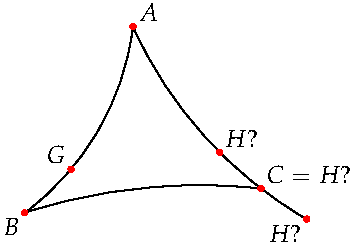
\includegraphics{basic-aaa}
   \end{minipage}
\end{enumerate}
\end{exercises}


\clearpage


\subsection{Omega-triangles}

\begin{minipage}[t]{0.7\linewidth}\vspace{-5pt}
Recall that limiting parallels (Definition \ref{defn:limparallel}) `meet' at an omega-point.

\begin{defn}{}{}
An \emph{omega-triangle} or \emph{ideal-triangle} is a `triangle' one or more of whose vertices is an omega-point. At least two of the sides of an omega-triangle form a pair of limiting parallels.
\end{defn}

The three types of omega-triangle depend on how many omega-points they have. In the picture, $\triangle PQ\Omega$ has one omega-point, $\triangle P\Omega\Theta$ has two and $\triangle \Omega\Theta\Xi$ three!
\end{minipage}\hfill\begin{minipage}[t]{0.28\linewidth}\vspace{-5pt}
\flushright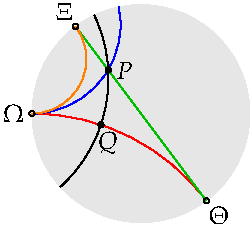
\includegraphics{omega-example}
\end{minipage}\smallbreak
Amazingly, many of the standard results of absolute geometry also apply to omega-triangles! The first can be thought of as the AAA congruence theorem where one `angle' is zero.

\begin{thm}{Angle-Angle Congruence for Omega-triangles}{}
Suppose $\triangle PQ\Omega$ and $\triangle RS\Theta$ are omega-triangles with a single omega-point. If the the angles are congruent in pairs
\[\angle PQ\Omega \cong\angle RS\Theta \qquad \angle QP\Omega \cong\angle SR\Theta\]
then the finite sides of each triangle are also congruent: $\cl{PQ}\cong\cl{RS}$.
\end{thm}

It doesn't really make sense to speak of the `infinite' sides, or the `angles' at omega-points, being congruent. However, if one defines congruence in terms of isometries (Section \ref{sec:hyperiso}), then this idea is more reasonable. %As with all these arguments, remember that your goal is simply follow them, not to create such on your own!

\begin{proof}
Transfer $\angle SR\Theta$ to $P$ and choose $T\in\ray{PQ}$ such that $\cl{PT}\cong\cl{RS}$. If $T=Q$ we are done.\par
\begin{minipage}[t]{0.7\linewidth}\vspace{-5pt}
Otherwise, WLOG assume $\cl{PQ}<\cl{PT}$. The hypothesis states that the \textcolor{orange}{marked orange angles} at $Q$ and $T$ are congruent.\smallbreak
Let $M$ be the midpoint of $\cl{QT}$ and drop the perpendicular to $\lin{Q\Omega}$ at $N$.\smallbreak
Choose $L\in\lin{\Omega T}$ on the opposite side of $\overleftrightarrow{QT}$ to $N$ such that $\textcolor{Green}{\cl{TL}\cong\cl{NQ}}$.\smallbreak
The \textcolor{red}{red angles} at $Q,T$ are congruent, as are the pairs of green and blue lines: SAS says $\triangle MQN\cong\triangle MTL$, whence $M$ lies on $\cl{LN}$ and we have a right-angle(!) at $L$.\smallbreak
The angle of parallelism of $L$ relative to $\lin{QN}$ is now \ang{90}: contradiction.\medbreak
There are several other possible orientations:
\begin{itemize}\itemsep0pt
  \item $T$ could lie on the same side of $Q$ as $P$ but the resulting argument is the same after reversing the roles of $Q$ and $T$.
  \item $N$ could lie on the opposite side of $Q$ from $\Omega$. In this case SAS is applied to the same triangles but with respect to the congruent \emph{orange} angles.
\end{itemize}\vspace{-12pt}
\end{minipage}\begin{minipage}[t]{0.3\linewidth}\vspace{0pt}
\flushright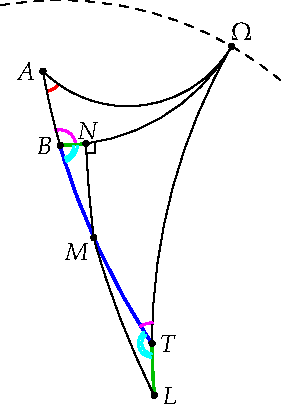
\includegraphics{basic-ext3}
\end{minipage}\par
\begin{itemize}\parsep0pt
  \item In the special case that $N=Q$, the orange angles are right-angles and the same contradiction appears.\qedhere
\end{itemize}
\end{proof}

\goodbreak


\begin{thm}{Exterior Angle Theorem for Omega-Triangles}{exthyp}
Suppose $\triangle QT\Omega$ has a single omega-point. Extend $\cl{TQ}$ to $P$. Then $\angle PQ\Omega>\angle QT\Omega$.
\end{thm}

\begin{tcolorbox}[proofstyle, lower separated=false, sidebyside, sidebyside align=top seam, sidebyside gap=0pt, righthand width=0.27\linewidth]
\emph{Proof.}\quad We show that the other cases are impossible.\medbreak
To see that $\angle PQ\Omega$ and $\angle QT\Omega$ cannot be congruent, consider the picture in the proof of the AA congruence theorem. The orange angles cannot be congruent since the entire picture is a contradiction!\medbreak
If $\angle PQ\Omega<\angle QT\Omega$, then we have the picture on the right. The goal is to create a triangle contradicting the usual exterior angle theorem.\smallbreak
Transfer $\textcolor{Green}{\angle QT\Omega}$ to $Q$ to obtain $\ray{QX}$ \emph{interior} to $\angle TQ\Omega$.\smallbreak
Since $\lin{Q\Omega}$ is a limiting parallel to $\lin{T\Omega}$, the Fundamental Theorem (\ref{thm:hyperfund}) says that $\ray{QX}$ intersects $\cl{T\Omega}$ at a point $Y$.\smallbreak
But now $\triangle QTY$ contradicts the standard exterior angle theorem.
\tcblower
\flushright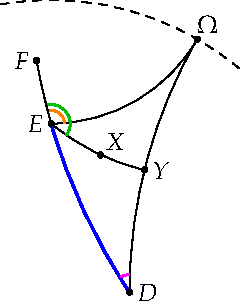
\includegraphics{basic-ext4}\\\hfil\qedsymbol
\end{tcolorbox}

The final congruence theorem is an exercise based on the previous picture.

\begin{cor}{Side-Angle Congruence for Omega-triangles}{}
Suppose $\triangle QT\Omega$ and $\triangle RS\Theta$ have a single omega-point. If $\angle QT\Omega \cong\angle RS\Theta$ and $\cl{QT}\cong\cl{RS}$ then $\angle TQ\Omega \cong\angle SR\Theta$.
\end{cor}

A triangle with one omega-point only has three pieces of data: two finite angles and one finite edge. The AA and SA congruence theorems say that two of these determine the third.

\boldsubsubsection{Other observations}

\emph{Pasch's Axiom}:\quad Versions of this are \emph{theorems} for omega-triangles.
\begin{itemize}
  \item If a line crosses a side of an omega-triangle and does not pass through any vertex (including $\Omega$), then it must pass through exactly one of the other sides.
  \item (\emph{Omega Crossbar Thm})\lstsp If a line passes through an interior point and exactly one vertex (including $\Omega$) of an omega-triangle, then it passes through the opposite side. This is partly embedded in the proof of Theorem \ref{thm:exthyp}.
\end{itemize}

% \emph{`Angle' Congruence}:\quad One could argue that omega-triangles with two omega-points and a single congruent angle are congruent. This statement is essentially vacuous as there is nothing to check: all sides have infinite length and the only real angles are assumed to be congruent! As before, once we have the machinery of isometries it makes more sense to describe such `triangles' as congruent.\medbreak

\emph{Perpendicular Distance and the Angle of Parallelism}:\quad Applied to right-angled omega-triangles, the AA and SA congruence theorems prove that the angle of parallelism is a bijective function of the perpendicular distance. Moreover, by transferring the right-angle to the positive $x$-axis and the other vertex to the origin, we obtain precisely the arrangement in Exercise \ref*{sec:hypparallel}.\ref{exs:angparallelism}, therefore completing the proof of Corollary \ref{cor:parangleformula}.




%  Below, we demonstrate the exterior angle theorem in such a situation and a special `Side-Angle' congruence theorem. It can also be shown that Pasch's axiom applies to omega-triangles:
% 
% It is important to note that these are \emph{Theorems} not \emph{Axioms} in hyperbolic geometry!

% \begin{thm}[Pasch's axiom for omega-triangles]
% If $\triangle PQ\Omega$ is an omega-triangle and a line $\ell$ passes through one of the vertices (including $\Omega$) and an interior point of the triangle, then it also passes through the opposite side.
% \end{thm}
% 
% \begin{proof}
% There are two cases.
% \begin{enumerate}
%   \item If $\ell$ passes through $P$ and an interior point, then it must intersect $\cl{P\Omega}$ by an argument similar to Theorem \ref{thm:hyperfund}.
%   \item Suppose that $\ell$ passes through $\Omega$ and an interior point $I$. Then $\ell=\overleftrightarrow{I\Omega}$ is a limiting parallel to both $\cl{P\Omega}$ and $\cl{Q\Omega}$. By part 1, the line $\overleftrightarrow{PI}$ meets $\cl{Q\Omega}$ at a point $J$. The fact that $\ell$ crosses $\cl{PQ}$ is now a consequence of Pasch's axiom for $\triangle PQJ$.
%   \hfill\qedhere
% \end{enumerate}
% \end{proof}





% \begin{thm}[Side-Angle congruence for Omega-triangles]
% Suppose that $\triangle PQ\Omega$ and $\triangle AB\Xi$ are two omega-triangles for which $\angle PQ\Omega\cong\angle AB\Xi$ and $\cl{PQ}\cong\cl{AB}$. Then $\angle QP\Omega\cong\angle BA\Xi$.
% \end{thm}
% 
% \begin{minipage}[t]{0.7\linewidth}\vspace{0pt}
% \begin{proof}
% If not, suppose WLOG that the measure of one angle $\angle QP\Omega$ is greater than $\angle BA\Xi$. We can then create a unique ray $\ray{PX}$ internal to $\angle QP\Omega$ for which $\angle BA\Xi\cong\angle QPX$. Pasch's axiom/theorem for omega-triangles says the ray intersects $\cl{Q\Omega}$, whence we may assume that $X$ lies on $\cl{Q\Omega}$. But then $\triangle PQX$ is congruent to $\triangle AB\Xi$ by angle-side-angle! This is gibberish: a finite triangle (with \emph{finite} side lengths) cannot be congruent to an omega-triangle. 
% \end{proof}
% 
% One can also prove a special `angle-angle' congruence for omega-triangles with one-omega point: if the pairs of `non-zero' angles are congruent, then so are the only `finite' sides.
% \end{minipage}\begin{minipage}[t]{0.3\linewidth}\vspace{0pt}
% \flushright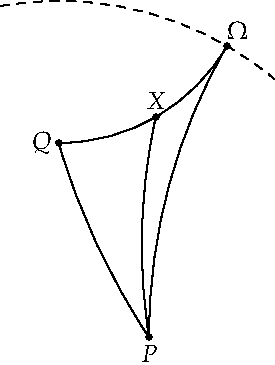
\includegraphics{basic-sa}
% \end{minipage}



% 
% More strictly: if triangle has hyperbolic radius $d$, then $r=\frac{e^d-1}{e^d+1}=\tanh\frac d2$. Can then be seen that
% \[\theta=2\tan^{-1}\frac{\operatorname{sech}(d/2)}{\sqrt 3}\]

\begin{exercises}
\exstart Let $\triangle PQ\Omega$ be an omega-triangle. Prove that $\measuredangle PQ\Omega+\measuredangle QP\Omega< \ang{180}$
\begin{enumerate}\setcounter{enumi}{1}
  \item Let $\ell$ and $m$ be limiting parallels. Explain why they cannot have a common perpendicular.
  
  \item Prove the Side-Angle congruence theorem for omega-triangles with one omega-point.
  
  \item What would an `omega-triangle' look like in Euclidean geometry? Comment on the three results in this section: are they still true?
 \end{enumerate}
\end{exercises}

\clearpage

	

\subsection{Area and Angle-defect}\label{sec:hyparea}

We turn toone of the triumphs of Johann Lambert: the relationship between the sum of the angles in a triangle and its \emph{area.} We start with a loose axiomatization of area as a relative measure and define a useful quantity. Until explicitly stated otherwise, we work in \emph{absolute geometry.}

\begin{description}
	\item[Axiom I] Two geometric figures have the same area if and only if they may be sub-divided into finitely many pairs of mutually congruent triangles.\footnote{To allow infinitely many infinitesimal sub-triangles would require ideas from calculus and complicate our discussion.}
	\item[Axiom II] The area of a triangle is positive.
	\item[Axiom III] The area of a union of disjoint figures is the sum of the areas of the figures.
\end{description}

\begin{defn}{Angle defect}{}
Let $\Sigma_\triangle$ be the sum of the angles in a triangle. Measured in radians, the \emph{angle-defect} of $\triangle$ is $\pi-\Sigma_\triangle$.
\end{defn}

Since triangles have angle-sum $\le\pi$ (Saccheri-Legendre (Thm \ref{thm:saccleg})), it follows that
\[0\le\pi-\Sigma_\triangle\le\pi\]
In Euclidean geometry the defect is always zero, while in hyperbolic geometry the defect is strictly positive (Theorem \ref{thm:hyptriangle}). A `triangle' with three omega-points would have defect $\pi$.

\begin{minipage}[t]{0.74\linewidth}\vspace{0pt}
\begin{lemm}{}{}
Angle-defect is additive: If a triangle is split into two sub-triangles, then the defect of the whole is the sum of the defects of the parts.
\end{lemm}

This is immediate from the picture:
\[\left[\pi-(\alpha+\gamma+\epsilon)\right]+\left[\pi-(\beta+\delta+\zeta)\right]=\pi-(\alpha+\beta+\gamma+\delta)\]
since $\epsilon+\zeta=\pi$. Notice that angle-\emph{sum} is not additive!
\end{minipage}\hfill\begin{minipage}[t]{0.25\linewidth}\vspace{-15pt}
\flushright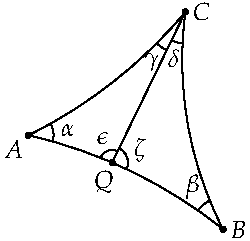
\includegraphics{area-defect}
\end{minipage}



\begin{thm}{Area determines angle-sum in \emph{absolute geometry}}{areatoanglesum}
If two triangles have the same area, then their angle-sums are identical.
\end{thm}
Of course this trivial in Euclidean geometry where all triangles have the same angle-sum!


\begin{proof}
The lemma provides the induction step: if $\triangle_1$ and $\triangle_2$ have the same area, then their interiors are disjoint unions of a finite collection of mutually congruent triangles:
\[\triangle_1=\bigcup_{k=1}^n\triangle_{1,k}\quad\text{and}\quad \triangle_2=\bigcup_{k=1}^n\triangle_{2,k}\quad\text{where}\quad \triangle_{1,k}\cong\triangle_{2,k}\]
Each pair $\triangle_{1,k},\triangle_{2,k}$ has the same angle-defect, whence the angle-defects of $\triangle_1$ and $\triangle_2$ are equal:
\[\operatorname{defect}(\triangle_1)=\sum_{k=1}^n\operatorname{defect}(\triangle_{1,k}) =\sum_{k=1}^n\operatorname{defect}(\triangle_{2,k}) =\operatorname{defect}(\triangle_2)\tag*{\qedhere}\]
\end{proof}

\goodbreak


\boldsubsubsection{Angle-sum determines area in \emph{hyperbolic geometry}}

The converse relies on a reversible construction relating triangles and Saccheri quadrilaterals. The construction itself is valid in absolute geometry, even though the ultimate conclusion that angle-sum determines area is not.

\begin{lemm}{}{quadtricorr}
% To every triangle there corresponds a Saccheri quadrilateral with the same area and whose summit angles sum to the angle-sum of the triangle. Explicitly:
\exstart Given $\triangle ABC$, choose a side $\cl{BC}$. Bisect the remaining sides at $E,F$ and drop perpendiculars from $A$, $B$, $C$ to $\lin{EF}$. Then $HICB$ is a Saccheri quadrilateral with base $\cl{HI}$.\vspace{-5pt}
\begin{enumerate}\setcounter{enumi}{1}
  %\item Given a triangle $\triangle ABC$, choose a side $\cl{BC}$. Bisect the remaining sides at $E,F$ and drop perpendiculars from $A,B,C$ to $\lin{EF}$. Then $HICB$ is a Saccheri quadrilateral with base $\cl{HI}$.
  \item Conversely, given a Saccheri quadrilateral $HICB$ with summit $\cl{BC}$, let $A$ be any point such that $\lin{HI}$ bisects $\cl{AB}$ at $E$. Then the intersection $F=\lin{HI}\cap\cl{AC}$ is the midpoint of $\cl{AC}$.
\end{enumerate}
\begin{minipage}[t]{0.6\linewidth}\vspace{-5pt}
Both constructions yield the same picture and the following conclusions:\vspace{-5pt}
  \begin{itemize}
    \item The triangle and quadrilateral have equal area.
    \item The sum of the summit angles of the quadrilateral equals the angle sum of the triangle.
  \end{itemize}
  We've chosen $\cl{BC}$ to be the longest side of $\triangle ABC$; this isn't necessary, though it helpfully forces $E,F$ to lie between $H,I$.
\end{minipage}\hfill\begin{minipage}[t]{0.39\linewidth}\vspace{-15pt}
\flushright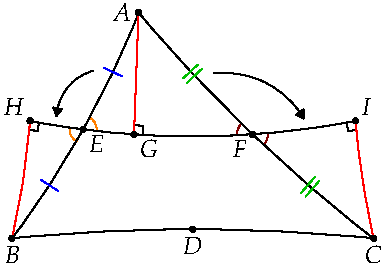
\includegraphics{area-saccheri4}
\end{minipage}
\end{lemm}


\begin{proof}
\begin{enumerate}
  \item By two applications of the SAA congruence theorem (follow the arrows\ldots)\vspace{-3pt}
  \[\triangle BEH\cong\triangle AEG\text{ \ and \ }\triangle CFI\cong\triangle AFG\]
  \begin{minipage}[t]{0.57\linewidth}\vspace{-11pt}
  We conclude that $\textcolor{red}{\cl{BH}\cong\cl{AG}\cong\cl{CI}}$ whence $HICB$ is a Saccheri quadrilateral. The area and angle-sum correspondences are immediate from the picture.
  \item Suppose the midpoint of $\cl{AC}$ were at $J\neq F$. By part 1, we may create a new Saccheri quadrilateral with base $\cl{BC}$ using the midpoints $E,J$.\smallbreak
  The perpendicular bisector of $\cl{BC}$ (at $D$) bisects the bases of both Saccheri quadrilaterals perpendicularly (Lemma \ref{lemm:saccheribasic}), creating $\triangle EUV$ with two right-angles: contradiction.
	\end{minipage}\begin{minipage}[t]{0.43\linewidth}\vspace{-20pt}
	\flushright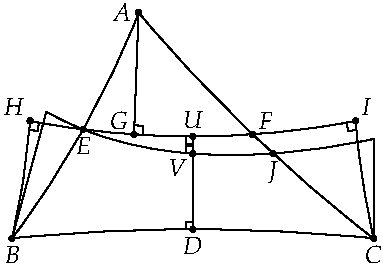
\includegraphics{area-saccheri5}\qedhere
	\end{minipage}%\par\vspace{-8pt}
	%\qedhere
\end{enumerate}
\end{proof}

We now prove a special case of the main result.

\begin{lemm}{}{anglesumarea}
Suppose \emph{hyperbolic} triangles $\triangle ABC$ and $\triangle PQR$ have congruent sides $\cl{BC}\cong\cl{QR}$ and the same angle-sum. Then the triangles have the same area.
\end{lemm}


\begin{proof}
Construct the quadrilaterals corresponding to $\triangle ABC$ and $\triangle PQR$ with summits $\cl{BC}\cong\cl{QR}$. These have congruent summits \emph{and} summit angles: by Exercise \ref*{sec:hypparallel}.\ref{exs:saccherisummitcong} they are congruent.
\end{proof}

The final observation is what makes this special to \emph{hyperbolic} geometry. In the Euclidean case, Saccheri quadrilaterals are \emph{rectangles}: congruent summits do not force congruence of the remaining sides.\goodbreak

\begin{thm}{}{arealemm2}
In hyperbolic geometry, if $\triangle ABC$ and $\triangle PQR$ have the same angle-sum then they have the same area.
\end{thm}

\begin{proof}
If the triangles have a congruent pair of edges, we are done by the previous result. Otherwise, we create a new triangle $\triangle LBC$ which matches the same Saccheri quadrilateral as $\triangle ABC$.\smallbreak
Otherwise, WLOG suppose $\nm{AB}<\nm{PQ}$ and construct the Saccheri quadrilateral with summit $\cl{BC}$. Select $K$ on $\lin{EF}$ such that $\nm{BK}=\frac 12\nm{PQ}$ and extend such that $K$ is the midpoint of $\cl{BL}$.\par
\begin{minipage}[t]{0.6\linewidth}\vspace{0pt}
\begin{itemize}
  \item By Lemma \ref{lemm:quadtricorr},
  \[\operatorname{Area}(\triangle LBC)=\operatorname{Area}(HICB)=\operatorname{Area}(\triangle ABC)\]
  \item By Theorem \ref{thm:areatoanglesum}, $\triangle LBC$ has the same angle-sum as $\triangle ABC$ and thus $\triangle PQR$.
  \item $\triangle LBC$ and $\triangle PQR$ share a congruent side ($\cl{LB}\cong\cl{PQ}$) and have the same angle-sum. Lemma \ref{lemm:anglesumarea} says their areas are equal.
\end{itemize}
\end{minipage}\hfill\begin{minipage}[t]{0.39\linewidth}\vspace{-12pt}
\flushright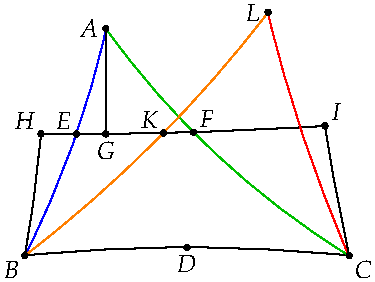
\includegraphics{area-saccheri9}\qedhere
\end{minipage}
\end{proof}

Since both area and angle-\emph{defect} are additive, we immediately conclude:

\begin{cor}{}{hypareaangle}
The angle-defect of a hyperbolic triangle is an additive function of its area: by normalizing the definition of area,\footnotemark{} we may conclude that
\[\pi-\Sigma_\triangle=\operatorname{Area}\triangle\]
\end{cor}

\footnotetext{We have really only proved that $\pi-\Sigma_\triangle\propto\operatorname{Area}\triangle$. However, it can be seen that these quantities are equal if we use the area measure arising naturally from the hyperbolic distance function (see page \pageref{pg:hypareaext}).\smallbreak
 The corollary is a special case of the famous Gauss--Bonnet theorem from differential geometry: for any triangle on a surface with Gauss curvature $K$, we have
\[\Sigma_\triangle-\pi=\iint_\triangle K\,\dA\]
The three special constant-curvature examples of this result are:
\begin{description}
\item[Euclidean space] This is \emph{flat} ($K=0$) so the angle-defect is always zero.
\item[Hyperbolic space] This has \emph{constant negative curvature} $K=-1$, and the area $\iint_\triangle\dA$ is precisely the angle-defect $\pi-\Sigma_\triangle$.
\item[Spherical geometry] A sphere of radius 1  has \emph{constant positive curvature} $K=1$, and the area of a triangle is its angle-\emph{excess} $\Sigma_\triangle-\pi$. 
\end{description}
The Gauss--Bonnet theorem is often the capstone result of an undergraduate course on differential geometry.}


Note finally how the AAA congruence (Theorem \ref{thm:hyptriangle}, part 3) is related to the corollary:
	\[\begin{array}{ccc}
	\triangle ABC\cong \triangle DEF & \overset{\text{AAA}}{\iff} & \text{angles congruent in pairs}\\[5pt]
	\Downarrow & & \Downarrow\\
	\text{equal area} & \overset{\text{Cor}}{\iff} & \text{same angle-defect}
	\end{array}\]
	
	\goodbreak

\begin{example*}{\ref{ex:hypisosceles}, cont}{}
The isosceles right-triangle with vertices $O$, $P=(\frac 12,0)$ and $Q=(0,\frac 12)$ has angle-sum and area
\[\frac\pi 2+2\tan^{-1}\frac 35\approx \ang{151.93}\implies \operatorname{area}=\pi-\left(\frac\pi 2+2\tan^{-1}\frac 35\right) =\frac\pi 2-2\tan^{-1}\frac 35\approx 0.490\]
A Euclidean triangle with the same vertices has area $\frac 12\cdot\frac 12\cdot\frac 12=\frac 18=0.125$.\par

\begin{minipage}[t]{0.7\linewidth}\vspace{0pt}
Generalizing this (Exercise \ref*{sec:hyp-models}.\ref{exs:isorighthypextended}), the triangle with vertices $O,P=(c,0)$ and $Q=(0,c)$ has area
\[\pi-\left(\frac\pi 2+2\tan^{-1}\frac{1-c^2}{1+c^2}\right)=\frac\pi 2-2\tan^{-1}\frac{1-c^2}{1+c^2}\]
As expected, $\lim\limits_{c\to 0^+}\text{area}(c)=0$. In the other limit, the triangle becomes an omega-triangle with two omega-points and $\lim\limits_{c\to 1^-}\text{area}(c)=\frac\pi 2$: an infinite `triangle' with finite `area'!
\end{minipage}\hfill\begin{minipage}[t]{0.29\linewidth}\vspace{0pt}
\flushright\begin{tabular}{c@{}}
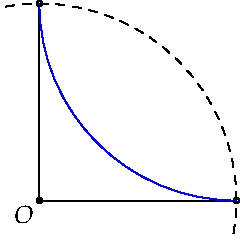
\includegraphics{area-iso}\\
The limit $c\to 1^-$
\end{tabular}
\end{minipage}
\end{example*}\vfil

Our discussion in fact provides an explicit method for cutting a triangle into sub-triangles and rearranging its pieces to create a triangle with equal area.

\begin{center}
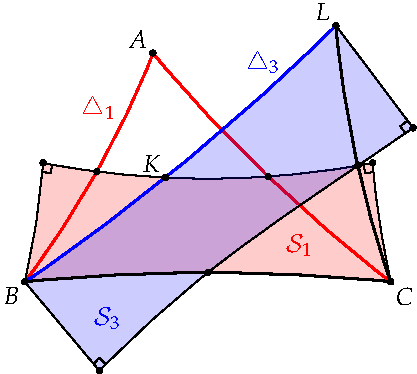
\includegraphics{area-saccheri10}\qquad\qquad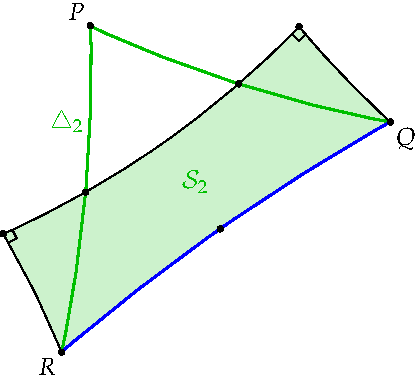
\includegraphics{area-saccheri8}
\end{center}

Suppose $\textcolor{red}{\triangle_1}$ and $\textcolor{Green}{\triangle_2}$ have equal area and construct the quadrilaterals $\textcolor{red}{\cS_1}$ and $\textcolor{Green}{\cS_2}$. Let $L,K$ be chosen so that $\textcolor{blue}{\cl{BL}\cong\cl{QR}}$ and $K$ is the midpoint of $\textcolor{blue}{\cl{BL}}$. We now have:
\begin{itemize}
  \item $\textcolor{red}{\triangle_1}, \textcolor{Green}{\triangle_2}, \textcolor{blue}{\triangle_3}, \textcolor{red}{\cS_1}, \textcolor{Green}{\cS_2}, \textcolor{blue}{\cS_3}$ have the same area.
  \item The summit angles of $\textcolor{red}{\cS_1}, \textcolor{Green}{\cS_2}, \textcolor{blue}{\cS_3}$ are congruent (half the angle-sum of each triangle).
  \item $\textcolor{Green}{\cS_2}, \textcolor{blue}{\cS_3}$ are \emph{congruent} since they have congruent summits and summit angles.
\end{itemize}

% All three triangles now have the same area, as do the Saccheri quadrilaterals $\cS_1$, $\cS_2$, and $\cS_3$.\smallbreak
% Moreover, all three Saccheri quadrilaterals have the same summit angles. Moreover, $\cS_2$ and $\cS_3$ are \emph{congruent} since they have congruent summits and the same area (Exercise \hyperref[exs:saccherisummitarea]{\ref*{sec:hyparea}.\ref*{exs:saccherisummitarea}}).
We can now follow the steps in Lemma \ref{lemm:quadtricorr} to transform $\textcolor{red}{\triangle_1}$ to $\textcolor{Green}{\triangle_2}$:
\[\textcolor{red}{\triangle_1}\to \textcolor{red}{\cS_1}\to \textcolor{blue}{\triangle_3}\to \textcolor{blue}{\cS_3}\cong \textcolor{Green}{\cS_2}\to \textcolor{Green}{\triangle_2}\]
where each arrow represents cutting off two triangles and moving them. Indeed this works even for triangles in Euclidean geometry: try it!

\goodbreak


\begin{exercises}
\exstart Use Corollary \ref{cor:hypareaangle} to find the area of the hyperbolic triangle with given vertices.
\begin{enumerate}\setcounter{enumi}{1}
  \item[]\begin{enumerate}
    \item $O=(0,0)$, $P=(\frac 12,\sqrt{\frac 5{12}})$ and $Q=(\frac 12,-\sqrt{\frac 5{12}})$.\par
		(\emph{You should already know the angles from previous exercises!})
    \item $O=(0,0)$, $P=(\frac 14,0)$, $Q=(0,\frac 12)$.
    \item $P=(r,0)$, $Q=\left(-\frac r2,\frac{\sqrt{3}r}2\right)$, $R=\left(-\frac r2,-\frac{\sqrt{3}r}2\right)$ where $0<r<1$.
	\end{enumerate}
	
	\item In the proof of Theorem \ref{thm:arealemm2}, explain why we can find $K$ such that $\nm{BK}=\frac 12\nm{PQ}$. 
	
	
% 	\item\label{exs:saccherisummitarea}\begin{enumerate}
%     \item Suppose that two Saccheri quadrilaterals share the same summit and have congruent sides. Prove that the quadrilaterals are congruent.
% 
%   	\item Suppose two Saccheri quadrilaterals have the same summit and area. Prove that they are congruent.
%   \end{enumerate}
%   
%   
%     
   \item Show that there is no finite triangle in hyperbolic geometry that achieves the maximum area bound $\pi$.\par
  (Hard!) For a challenge, try to prove that omega-triangles also satisfy the angle-defect formula: Area $=\pi-\Sigma_\triangle$, so that only triangles with three omega-points have maximum area.

	\item Let $\Omega_1,\ldots,\Omega_n$ be $n$ distinct omega-points arranged counter-clockwise around the boundary circle of the Poincaré disk. A region is bounded by the $n$ hyperbolic lines
	\[\overleftrightarrow{\Omega_1\Omega_2},\quad \overleftrightarrow{\Omega_2\Omega_3},\quad\ldots,\quad\overleftrightarrow{\Omega_n\Omega_1}\]
	What is the area of the region? Hence argue that the `area' of hyperbolic space is infinite.
  
  \item An omega-triangle has vertices $O=(0,0)$, $\Omega=(1,0)$ and $P=(0,h)$ where $h>0$.
  \begin{enumerate}
    \item Prove that the hyperbolic segment $\cl{P\Omega}$ is an arc of a circle with equation
    \[(x-1)^2+(y-k)^2=k^2\]
    for some $k>0$.
    \item Prove that the area of $\triangle OP\Omega$ is given by
		\[A(h)=\sin^{-1}\dfrac{2h}{1+h^2}\]
	\end{enumerate}

\end{enumerate}
\end{exercises}

\clearpage




\subsection{Isometries and Calculation}\label{sec:hyperiso}

There are (at least!) two major issues in our approach to hyperbolic geometry.

\begin{description}
	\item[Calculations are difficult] In analytic (Euclidean) geometry we typically choose the origin and orient axes to ease calculation. We'd like to do the same in hyperbolic geometry.
	\item[We assumed too much] We defined \emph{distance, angle} and \emph{line} separately, but these concepts are \emph{not independent}! In Euclidean geometry, the distance function, or \emph{metric,} defines angle measure via the dot product,\footnote{Writing $\nm{\vu}=\nm{PQ}$ for the length of a line segment, we see that for any $\vu,\vv$,
\[\vu\cdot\vv=\frac 12\left(\nm{\vu+\vv}^2-\nm\vu^2-\nm\vv^2\right)\]
so that the metric defines the dot product. Now define angle measure via $\vu\cdot\vv=\nm\vu\nm\vv\cos\theta$.} and (with some calculus) the arc-length of any curve. One then  proves that the paths of shortest length (\emph{geodesics}) are straight lines: the metric \emph{defines} the notion of line!
\end{description}


% \begin{minipage}[t]{0.6\linewidth}\vspace{0pt}
% \begin{lemm}{}{}
% \begin{enumerate}
%   \item Consider the Poincaré disk as the subset
%   \[D=\{z\in\C:\nm z<1\}\]
%   of the complex plane. If $z\in D\setminus\{0\}$, then the omega-points on the line joining $0$ and $z$ are $\Omega=\frac z{\nm z}$ and $\Theta=-\frac z{\nm z}$, whence
% 	\[d(0,z)=\nm{\ln\frac{\nm{0-\Omega}\nm{z-\Theta}}{\nm{0-\Theta}\nm{z-\Omega}}}=\ln\left(\frac{1+\nm z}{1-\nm z}\right)\]
% \end{enumerate}
% \end{lemm}
% \end{minipage}\begin{minipage}[t]{0.4\linewidth}\vspace{0pt}
% \flushright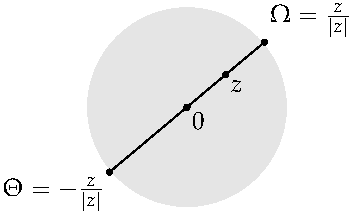
\includegraphics{isom-lemma}
% \end{minipage}


% {\itshape\begin{enumerate}\setcounter{enumi}{1}
%   \item Suppose a point lies a Euclidean distance $r$ and hyperbolic distance $\delta$ from the origin. Then
% 	\begin{gather*}
% 	\delta=\ln\left(\frac{1+r}{1-r}\right) =\cosh^{-1}\frac{1+r^2}{1-r^2},\qquad r^2=\frac{\cosh\delta-1}{\cosh\delta+1},\qquad r=\frac{e^\delta-1}{e^\delta+1} =\tanh\frac\delta 2
% 	\end{gather*}
% \end{enumerate}}
% One can observe the equivalence of the logarithm and inverse-cosh expressions for hyperbolic distance beginning to emerge.


Isometries provide a related remedy for these issues. To work with these we require an alternative definition of the Poincaré disk, and some facts (stated without proof) from complex analysis.

\begin{defn}[lower separated=false, sidebyside, sidebyside align=top seam, sidebyside gap=0pt, righthand width=0.3\linewidth]{}{hypdist2}
The \emph{Poincaré disk} is the set $D:=\{z\in\C:\nm z<1\}$ equipped with the distance function
\[d(z,w):=\nm{\ln\frac{\nm{z-\Omega}\nm{w-\Theta}}{\nm{z-\Theta}\nm{w-\Omega}}}\]
where $\Omega,\Theta$ are the omega-points for the hyperbolic line through $z,w$ (defined via circles).
\tcblower
\flushright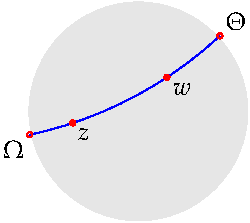
\includegraphics{isom-dist}
\end{defn}

We'll see later (Corollary \ref{cor:hypcosinerule}) that this is the same as the original cosh formula (page \pageref{lemm:distformula}); it is already easy to see that $d(z,0)=\ln\frac{1+\nm z}{1-\nm z}$ as in Lemma \ref{lemm:distformula}. Now we need some functions which play nicely with $d(z,w)$.


\begin{thm}{Möbius/fractional-linear transformations}{mobius}
If $a,b,c,d\in\C$ and $ad-bc\neq 0$, then the function $f(z)=\tfrac{az+b}{cz+d}$ has the following properties:
\begin{enumerate}
  \item (Invertibility)\lstsp $f:\C\cup\{\infty\}\to \C\cup\{\infty\}$ is bijective, with inverse $f^{-1}(z)=\tfrac{dz-b}{-cz+a}$.
  \item (Conformality)\lstsp If curves intersect, then their images under $f$ intersect at the same angle.
  \item (Line/circle preservation)\lstsp Every line/circle\footnotemark{} is mapped by $f$ to another line/circle.
  \item(Cross-ratio preservation)\lstsp Given distinct $z_1,z_2,z_3,z_4$, we have
	\[\frac{\big(f(z_1)-f(z_2)\big)\big(f(z_3)-f(z_4)\big)}{\big(f(z_2)-f(z_3)\big)\big(f(z_4)-f(z_1)\big)} =\frac{(z_1-z_2)(z_3-z_4)}{(z_2-z_3)(z_4-z_1)}\]
\end{enumerate}
\end{thm}

\footnotetext{In $\C\cup\{\infty\}$ a line is just a circle containing $\infty$\ldots}


\goodbreak

The isometries of the Poincaré disk are a subset of the Möbius transformations.

\begin{thm}{}{hypisomclass}
The \emph{orientation-preserving\footnotemark{} isometries} of the Poincaré disk have the form
\[f(z)=e^{i\theta}\frac{\alpha-z}{\cl\alpha z-1}\quad\text{where $\nm\alpha<1$ and $\theta\in[0,2\pi)$}\tag{$\ast$}\]
All isometries can be found by composing $f$ with complex conjugation (reflection in the real axis).
\end{thm}

\footnotetext{If $C$ is to the left of $\ray{AB}$, then $f(C)$ is to the left of $\ray{f(A)f(B)}$. This is the usual `right-hand rule.'} 


Referring to the properties in Theorem \ref{thm:mobius}:
\begin{enumerate}\itemsep0pt
  \item The isometries are precisely the set of Möbius transformations which map $D$ bijectively to itself; omega-points are also mapped to omega-points.
  \item Isometries preserve angles.
  \item The class of hyperbolic lines is preserved: any circle or line intersecting the unit circle at right-angles is mapped to another such (angle-preservation is used here). 
  \item If $\Omega,\Theta$ are the omega-points on $\lin{zw}$, then (by 2 and 3), $f(\Omega)$ and $f(\Theta)$ are the omega-points for the hyperbolic line through $f(z),f(w)$. Preservation of the cross-ratio says that $f$ is an isometry:
  \[d(f(z),f(w))=\nm{\ln\frac{\nm{f(z)-f(\Omega)}\nm{f(w)-f(\Theta)}}{\nm{f(z)-f(\Theta)}\nm{f(w)-f(\Omega)}}}= \nm{\ln\frac{\nm{z-\Omega}\nm{w-\Theta}}{\nm{z-\Theta}\nm{w-\Omega}}}=d(z,w)\]
\end{enumerate}

How does this help us compute? The isometry $f$ ($\ast$) moves $\alpha$ to the origin; one can then choose $\theta$ to orient whichever direction you like along the positive $x$-axis\ldots



% 
% \boldinline{Example}
% 
% Given $z=\frac 12(1+i)$, we have $r^2=\frac 12$, whence
% \[\delta=d(0,z)=\cosh^{-1}3=\ln\left(\frac{1+1/\sqrt 2}{1-1/\sqrt 2}\right)=\ln(3+2\sqrt 2)\]


\begin{example}{}{}
Let $P=\frac 12$ and $Q=\frac 23+\frac{\sqrt 2}3i$. Move $P$ to the origin using\par
\begin{minipage}[t]{0.74\linewidth}\vspace{-8pt}
an isometry with $\alpha=P$:
\begin{gather*}
f(z)=e^{i\theta}\frac{\alpha-z}{\cl\alpha z-1}=e^{i\theta}\frac{1-2z}{z-2} \implies f(P)=O\\
f(Q)=e^{i\theta}\frac{1-\frac 43-\frac{2\sqrt 2}3i}{\frac 23-2+\frac{\sqrt 2}3i} =-\frac{1+2\sqrt 2i}{-4+\sqrt 2i}e^{i\theta} =\frac{i}{\sqrt 2}e^{i\theta}
\end{gather*}
Choosing $e^{i\theta}=-i$ places $f(Q)=\frac 1{\sqrt 2}$ on the positive $x$-axis. Now check using our original definition of hyperbolic distance:
\end{minipage}\hfill
\begin{minipage}[t]{0.25\linewidth}\vspace{-20pt}
\flushright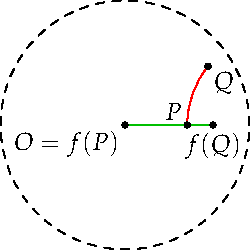
\includegraphics{calc-triangle2}
\end{minipage}\par\vspace{-4pt}
\begin{gather*}
\begin{aligned}
d(P,Q)&=\cosh^{-1}\left(1+\frac{2\nm{PQ}^2}{(1-\nm P^2)(1-\nm Q^2)}\right) =\cosh^{-1}\left(1+\frac{\frac 24}{(1-\frac 14)(1-\frac 23)}\right)\\
&=\cosh^{-1}3=\ln(3+2\sqrt 2)
\end{aligned}\\
\begin{aligned}
d(f(P),f(Q))&=\ln\frac{1+\frac 1{\sqrt 2}}{1-\frac 1{\sqrt 2}}=\ln\frac{\sqrt 2+1}{\sqrt 2-1}=\ln(3+2\sqrt 2)
\end{aligned}
\end{gather*}
The points really are the same distance apart! Indeed the hyperbolic segment \textcolor{red}{$\cl{PQ}$} (with equation $x^2+y^2-\frac 52x+1=0$) has been transformed by $f$ to a segment \textcolor{Green}{$\cl{f(P)f(Q)}$} of the $x$-axis.
\end{example}

\goodbreak

Recall (e.g.{} Example \ref{ex:hypisosceles}) how we previously computed angles. Isometries make this \emph{much} easier. 

\begin{example}{}{}
Given $A=-\frac i2$, $B=-\frac i5$ and $C=-\frac 1{5}(3+i)$, we find $d(A,B)$, $d(A,C)$ and $\measuredangle BAC$.\smallbreak
Start by moving $A$ to the origin and consider $f(B)$:
\[f(z)=e^{i\theta}\frac{-\frac i2-z}{\frac i2z-1} =\frac{2z+i}{2-iz}e^{i\theta} \qquad f(B)=\frac{-\frac{2i}5+i}{2-\frac 15}e^{i\theta} =\frac i3e^{i\theta}=\frac 13\]
where we chose $e^{i\theta}=-i$ to force $f(B)$ onto the positive $x$-axis (this is unnecessary). Thus\par
\begin{minipage}[t]{0.64\linewidth}\vspace{-10pt}
\[f(z)=\frac{2z+i}{z+2i}\implies f(C)=\frac{-\frac 25(3+i)+i}{-\frac 15(3+i)+2i}=\frac{1+i}2\]
By mapping $A$ to the origin, \textcolor{red}{two} \textcolor{blue}{sides} of the triangle are now \emph{Euclidean straight lines} and the computations are easy:
\begin{gather*}
  d(A,B)=d\bigl(O,f(B)\bigr)=\ln\frac{1+\frac 13}{1-\frac 13}=\ln 2\\
  d(A,C)=d\bigl(O,f(C)\bigr)=\ln\frac{1+\frac 1{\sqrt 2}}{1-\frac 1{\sqrt 2}}=2\ln (\sqrt 2+1)\\[-3pt]
  \measuredangle BAC=\arg\frac{1+i}2=\frac\pi 4
\end{gather*}
\end{minipage}\hfill
\begin{minipage}[t]{0.34\linewidth}\vspace{-2pt}
\flushright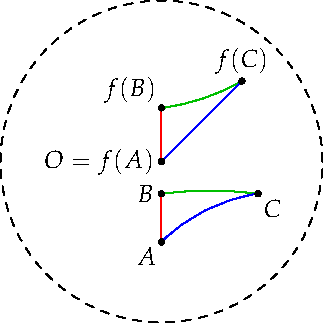
\includegraphics[scale=0.9]{calc-triangle}
\end{minipage}\bigbreak
%The picture hopefully makes clear the meaning of \emph{orientation-preserving}: $\triangle ABC$ was rotated and translated to obtain $\triangle f(A)f(B)f(C)$, but not reflected.
\end{example}



\boldinline{Interpretation of Isometries (non-examinable)}

As in Euclidean geometry, we can interpret isometries as rotations, reflections and translations. Here is the dictionary in hyperbolic space.\par

\begin{minipage}[t]{0.75\linewidth}\vspace{-3pt}
\begin{description}
\item[\normalfont\emph{Translations}] Move $\alpha$ to the origin via $T_{-\alpha}(z)=\frac{\alpha-z}{\cl\alpha z-1}$\par
The picture shows repeated applications of $T_{-\alpha}$ to seven initial points.\par
% To move the origin to $\alpha$, we need the inverse function
% \[T_{-\alpha}=\frac{-\alpha-z}{-\cl\alpha z-1}=\frac{\alpha+z}{\cl\alpha z+1}\]
Compose these to translate $\alpha$ to $\beta$:
\[T_{\beta}\circ T_{-\alpha}(z)=\frac{(\cl\alpha\beta-1)z+\alpha-\beta}{(\cl\alpha-\cl\beta)z+\alpha\cl\beta-1}\]

\item[\normalfont\emph{Rotations}] $R_\theta(z)=e^{i\theta}z$ rotates counter-clockwise around the origin. To rotate around $\alpha$, one computes the composition
	\[T_{\alpha}\circ R_\theta\circ T_{-\alpha}\]
	The picture shows repeated rotation by $\ang{30}=\frac\pi 6$ around $\alpha$.

\item[\normalfont\emph{Reflections}] $P_\theta(z)=e^{2i\theta}\cl z$ reflects across the line making angle $\theta$ with the real axis. Composition permits more general reflections, e.g.
	\[T_{\alpha}\circ P_\theta\circ T_{-\alpha}\]
\end{description}
\end{minipage}\hfill
\begin{minipage}[t]{0.24\linewidth}\vspace{-3pt}
\flushright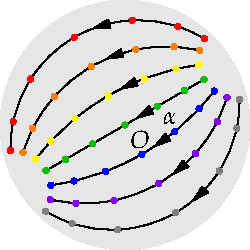
\includegraphics[scale=0.95]{isom-trans}\\
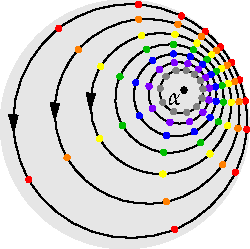
\includegraphics[scale=0.95]{isom-rotate}
\end{minipage}

\goodbreak





\boldsubsubsection{Hyperbolic Trigonometry\footnotemark}\footnotetext{Don't memorize these formulæ; in an exam, everything relevant will be given!}

The goal of trigonometry is to `solve' triangles: given minimal numerical data, we compute the remaining side lengths and angle measures. In hyperbolic geometry, the triangle congruence theorems (SAS, ASA, SSS, SAA \emph{and} AAA) provide suitable minimal data.\smallbreak

We start with a right-triangle, where we may suppose an isometry has already moved the right-angle to the origin and the other sides to the positive axes. The non-hypotenuse side lengths are\par
\begin{minipage}[t]{0.675\linewidth}\vspace{-8pt}
\[a=\ln\frac{1+p}{1-p}=\cosh^{-1}\frac{1+p^2}{1-p^2},\qquad b=\cosh^{-1}\frac{1+q^2}{1-q^2}\]
To measure the hypotenuse, apply another isometry to translate $p$ to the origin
\[f(z)=\frac{p-z}{pz-1} \implies f(iq)=\frac{p-iq}{ipq-1} \implies \nm{f(iq)}^2=\frac{p^2+q^2}{p^2q^2+1}\]
% But then
\end{minipage}\hfill\begin{minipage}[t]{0.3\linewidth}\vspace{0pt}
\flushright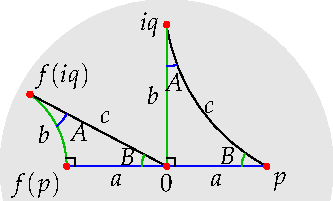
\includegraphics[scale=0.9]{isom-right}
\end{minipage}\medbreak
% \begin{gather*}
% f(iq)=\frac{p-iq}{ipq-1} =\frac{-p(1+q^2)+iq(1-p^2)}{p^2q^2+1}
% \implies \tan B=\frac{q(1-p^2)}{p(1+q^2)}\  \text{ and }\ \nm{f(iq)}^2=\frac{p^2+q^2}{p^2q^2+1}
% \end{gather*}
We therefore see that
\[\cosh c=\frac{1+\nm{f(iq)}^2}{1-\nm{f(iq)}^2}  =\frac{1+p^2+q^2+p^2q^2}{1-p^2-q^2+p^2q^2} =\frac{1+p^2}{1-p^2}\cdot\frac{1+q^2}{1-q^2} =\cosh a\cosh b\]
This is Pythagoras' Theorem for hyperbolic right-triangles!\smallbreak
Moreover, applying the hyperbolic identity $\sinh^2b=\cosh^2b-1$, we obtain
\[\sinh b=\frac{2q}{1-q^2}\implies
\tanh b=\frac{\sinh b}{\cosh b} =\frac{2q}{1+q^2}\]
Writing $f(iq)$ in real and imaginary parts allows us to find the slope
\[f(iq)=\frac{p-iq}{ipq-1} =\frac{-p(1+q^2)+iq(1-p^2)}{p^2q^2+1}\implies \tan B=\frac{q(1-p^2)}{p(1+q^2)}\]
Applying trig identities such as $\sec^2B=1+\tan^2B$, we finally conclude:

\begin{thm}{}{hyptrig}
In a hyperbolic right-triangle with adjacent $a$, opposite $b$, and hypotenuse $c$,
\begin{gather*}
\cos B=\frac{\tanh a}{\tanh c}\qquad \sin B=\frac{\sinh b}{\sinh c}\qquad \tan B=\frac{\tanh b}{\sinh a}\qquad \cosh c=\cosh a\cosh b
\end{gather*}
\end{thm}

\begin{cor}{Cosine rule}{hypcosinerule}
Apply the same argument to a triangle with vertices $0,p,qe^{iC}$ to obtain
\[\cosh c=\cosh a\cosh b-\sinh a\sinh b\cos C\]
Expressing the right-hand side in terms of $p,q$ ($\cosh a=\frac{1+p^2}{1-p^2}$, $\sinh a=\sqrt{\cosh^2\!a-1}=\frac{2p}{1-p^2}$, \ etc.) and applying the Euclidean cosine rule yields our original cosh-formula for distance (page \pageref{lemm:distformula}).
\end{cor}


\begin{cor}[lower separated=false, sidebyside, sidebyside align=top seam, sidebyside gap=0pt, righthand width=0.25\linewidth]{Sine Rule}{}
In a hyperbolic triangle,
\[\frac{\sinh a}{\sin A}=\frac{\sinh b}{\sin B}=\frac{\sinh c}{\sin C}\]
The picture shows the generic situation: simply apply Theorem \ref{thm:hyptrig} and equate the $\sinh h$-terms\ldots
\tcblower
\flushright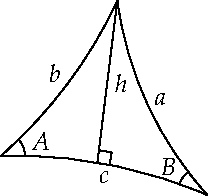
\includegraphics{isom-sine}
\end{cor}

Armed with these results, one can solve any hyperbolic triangle numerically given the information in one of the triangle congruence theorems. Admittedly ASA and the general AAA are very messy to compute with, but others are straightforward.

% ASA is two applications of the cosine rule for $\cosh a,\cosh b$, subs one in the other and apply the sine rule to obtain
% \[\tanh a=\frac{\sinh c}{\cos B\cosh c+\cot A\sin B}\]
% For AAA, square this and use $\coth^2a=1+\frac 1{\sinh^2a}=1+\frac{\sin^2C}{\sinh^2c\sin^2A}$ to obtain a quadratic for $\cosh c$ after multiplying out\ldots

\begin{examples}{}{}
\exstart (right-angled AAA)\lstsp A triangle has angles $\frac\pi 6,\frac\pi 4$ and $\frac\pi 2$: find its sides.
\begin{enumerate}\setcounter{enumi}{1}
  \begin{minipage}[t]{0.71\linewidth}\vspace{-10pt}
  \item[] Using the tan-formula,
  \begin{gather*}
  \frac 1{\sqrt 3}=\tan\frac\pi 6=\frac{\tanh b}{\sinh a}=\frac{\sinh b}{\sinh a\cosh b}\\
  1=\tan\frac\pi 4=\frac{\tanh a}{\sinh b}=\frac{\sinh a}{\cosh a\sinh b}
  \end{gather*}
  Now multiply together and use hyperbolic Pythagoras,
  \end{minipage}
  \begin{minipage}[t]{0.28\linewidth}\vspace{-20pt}
  \flushright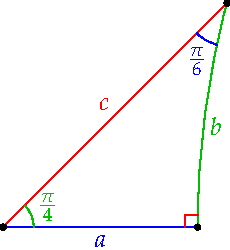
\includegraphics{isom-right2}
  \end{minipage}\par
  \[\frac 1{\sqrt 3}=\frac 1{\cosh a\cosh b}=\frac 1{\cosh c}\implies c=\cosh^{-1}\sqrt 3=\ln(\sqrt 3+\sqrt 2)\approx 1.1462\]
  We quickly see that $\sinh c=\sqrt{\cosh^2c-1}=\sqrt 2$, whence the sine-rule yields the other sides:
  \begin{gather*}
  \sinh b=\sin\frac\pi 4\cdot\frac{\sinh c}{\sin\pi}=1 \implies b=\sinh^{-1} 1 =\cosh^{-1}\sqrt 2\approx 0.8814\\
  \implies \cosh a=\frac{\cosh c}{\cosh b}=\sqrt{\frac 32} \implies a\approx 0.6565
  \end{gather*}
 

  \item (SAS)\quad A triangle has angle $C=\frac{\pi}3$ between sides $a=b=\cosh^{-1}2$. Find the remaining data.\smallbreak

	We have $\sinh a=\sinh b=\sqrt{\cosh^2\!a-1}=\sqrt 3$. By the cosine rule,
	\[\cosh c=2\cdot 2-\sqrt 3\sqrt 3\cdot \frac 12 =\frac 52\implies c=\cosh^{-1}\frac 52\]
	Finally, apply the sine rule:
	\[\sin B=\sin A=\frac{\sin C\sinh a}{\sinh c}=\frac{\sqrt 3}2\cdot\frac{\sqrt 3}{\sqrt{21}/2}=\frac 3{\sqrt{21}}=\sqrt{\frac 37}\]
 	The area of this triangle is therefore
 	\[\pi-\frac{\pi}3-2\sin^{-1}\sqrt{\frac 37}\approx 0.6669\]
\end{enumerate}
\end{examples}





\boldsubsubsection{Hyperbolic Tilings (just for fun!)}
The first example above can be used to make a regular tiling of hyperbolic space.\par

\begin{minipage}[t]{0.55\linewidth}\vspace{0pt}
Take eight congruent copies of the triangle and arrange them around the origin as in the picture. Now reflect the quadrilateral over each of its edges and repeat the process in all directions. We obtain a regular tiling of hyperbolic space comprising \emph{four-sided} figures with \emph{six} meeting at every vertex!\medbreak

In hyperbolic space, many different regular tilings are possible. Suppose such is to be made using regular $m$-sided polygons, $n$ of which are to meet at each vertex: each polygon comprises $2m$ copies of the fundamental right-triangle, whose angles are therefore $\frac\pi 2, \frac\pi m$ and $\frac\pi n$.
Since the angles sum to less than $\pi$ radians, we see that there exists a regular tiling of hyperbolic space whenever $m,n$ satisfy
\[\frac\pi 2+\frac\pi m+\frac\pi n<\pi\iff (m-2)(n-2)>4\]
The first example is $m=4$ and $n=6$, where the fundamental triangle is clear. In the second example four pentagons meet at each vertex and the interiors of the polygons have been colored. This was produced using the tools found
\href{http://www.malinc.se/noneuclidean/en/poincaretiling.php}{here} and \href{http://www.malinc.se/m/ImageTiling.php}{here}: have a play!\medbreak

The multitude of possible tilings in hyperbolic geometry is in contrast to Euclidean geometry, where a regular tiling requires \emph{equality}
\[(m-2)(n-2)=4\]
The three solutions $(m,n)=(3,6)$, $(4,4)$, $(6,3)$ correspond to the only tilings of Euclidean geometry by regular polygons (equilateral triangles, squares and hexagons). However, all can be scaled to arbitrary side-lengths. In hyperbolic geometry, there are infinitely many distinct tilings, but each has a unique side-length.\bigbreak

For related fun, look up M.C.\,Escher's \emph{Circle Limit} artworks, some of which are based on hyperbolic tilings.
If you want an excuse to play video games while pretending to study geometry, have a look at \href{http://www.roguetemple.com/z/hyper/}{Hyper Rogue}, which relies on (sometimes irregular) tilings.
\end{minipage}\begin{minipage}[t]{0.45\linewidth}\vspace{-20pt}
\centering
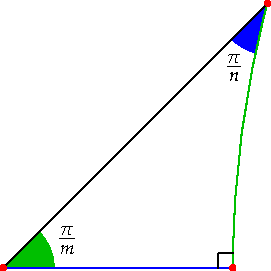
\includegraphics{isom-right3}\\
The fundamental triangle\bigbreak
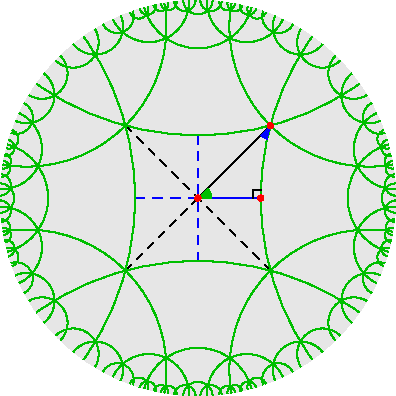
\includegraphics{isom-tiling}\\
$(m,n)=(4,6)$\bigbreak
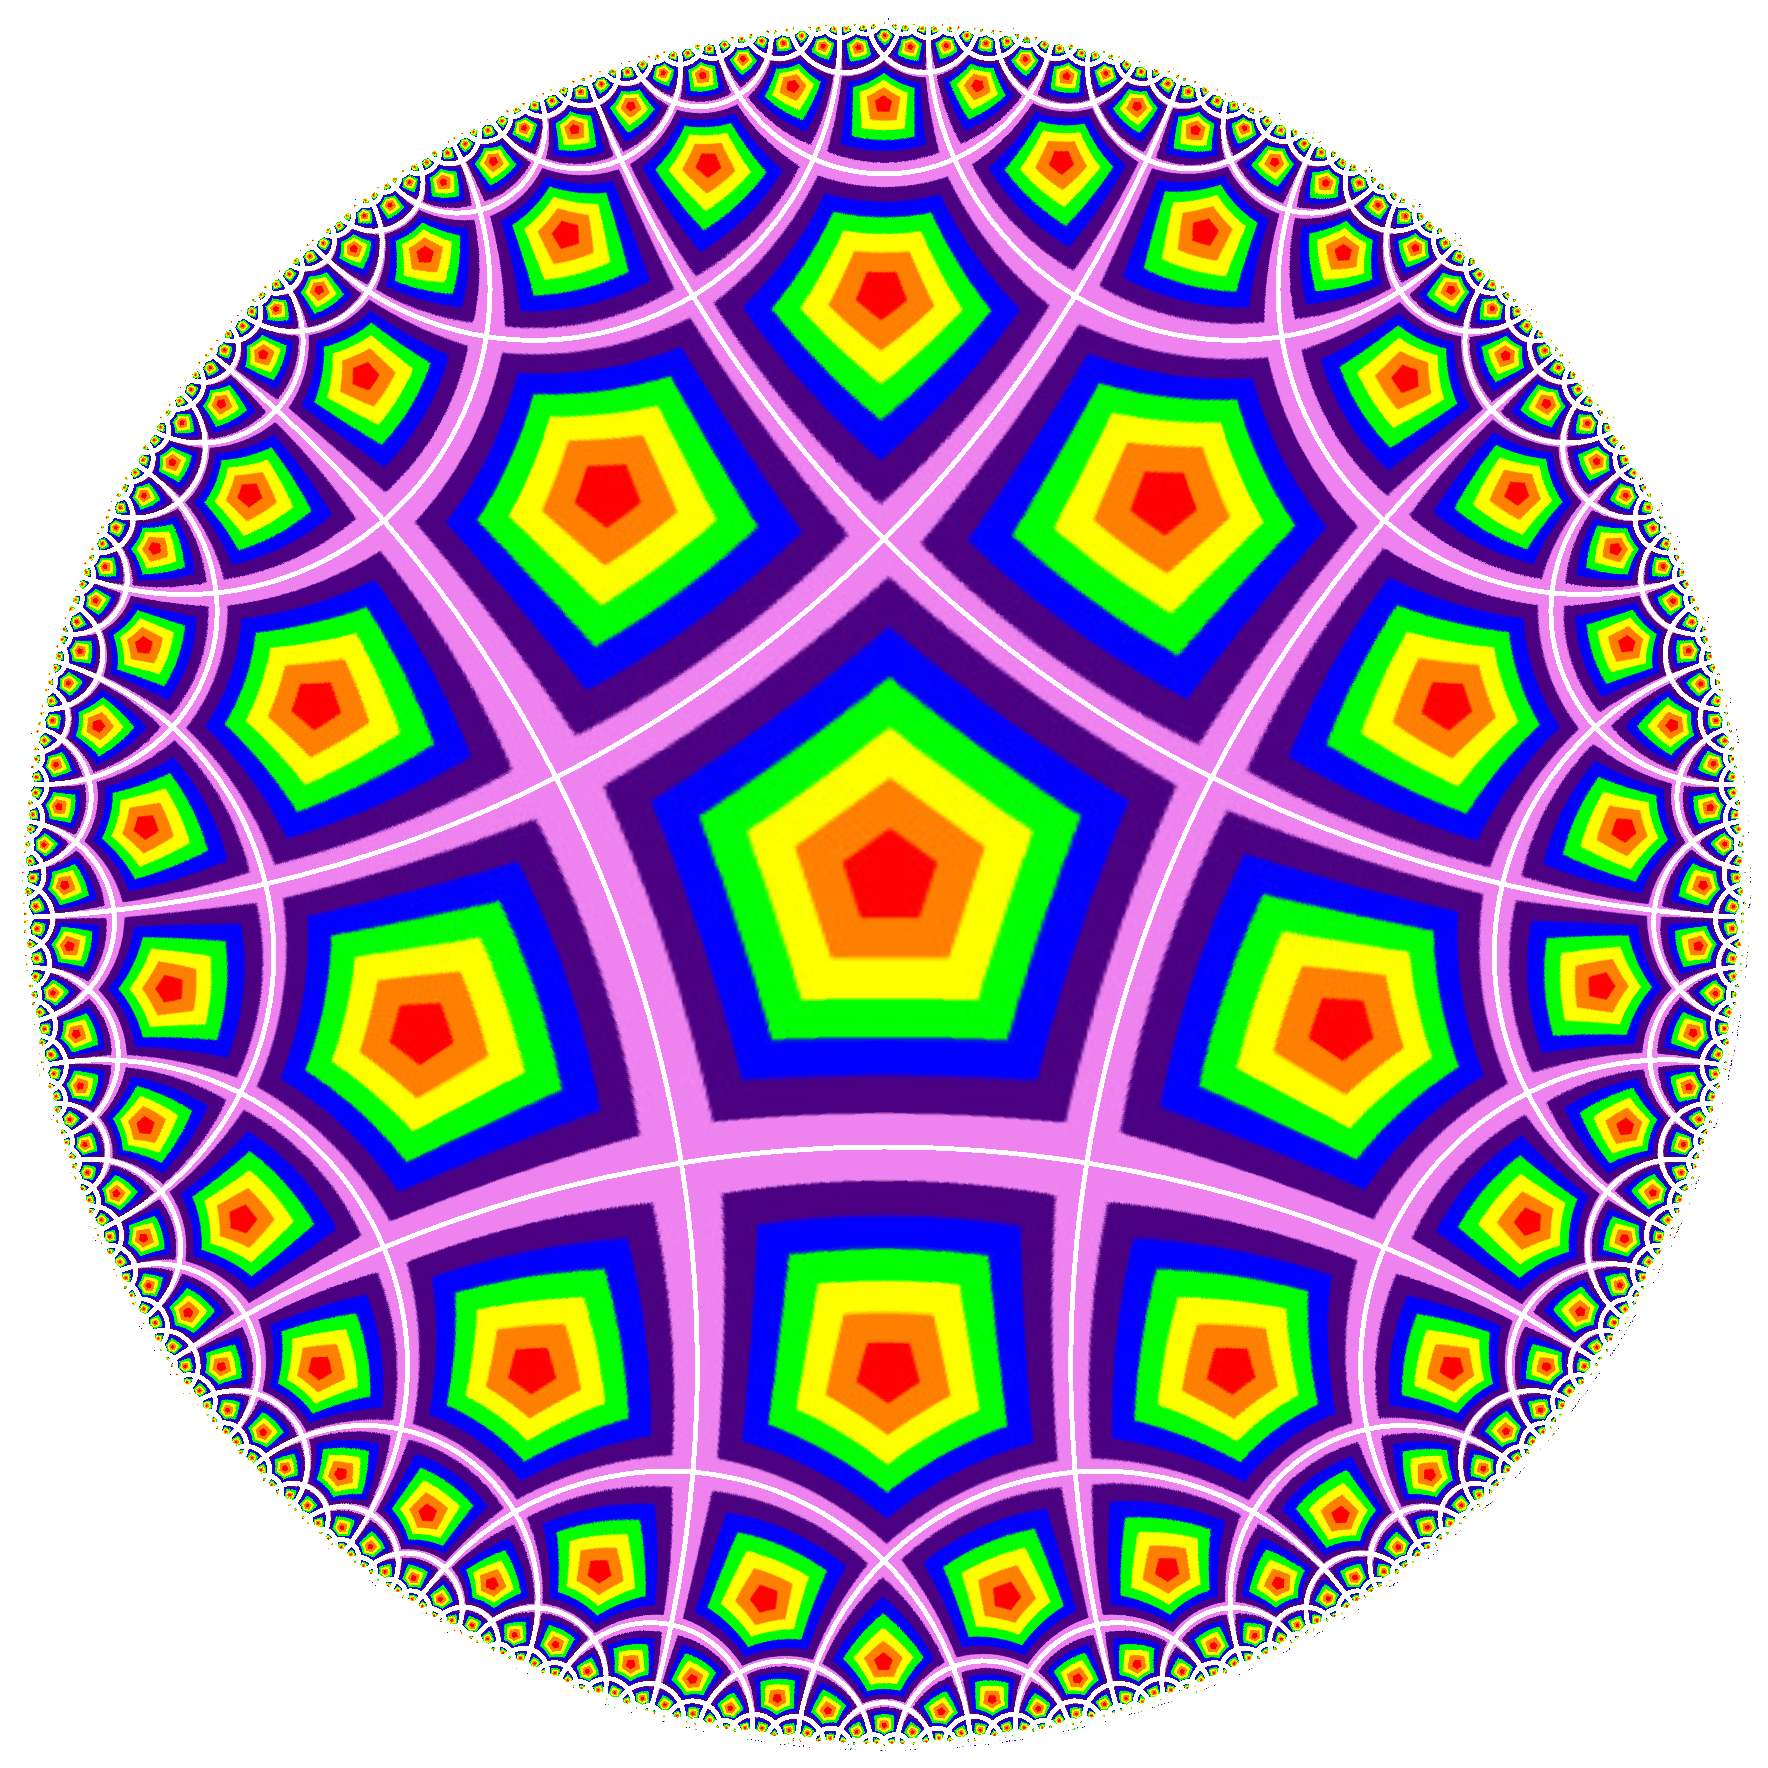
\includegraphics[scale=0.112]{tiling}\\
$(m,n)=(5,4)$
\end{minipage}\goodbreak



\begin{exercises}
\hangindent\leftmargini
1. \ Use Definition \ref{defn:hypdist2} to prove that $d(z,0)=\ln\frac{1+\nm z}{1-\nm z}$.
\begin{enumerate}\setcounter{enumi}{1}
  \item[](\emph{Hint: what are the omega-points for the line through $0$ and $z$?})
  
  \item Use an isometry to find angle $\measuredangle ABC$ when
  \[A=0,\quad B=\frac i2,\quad C=\frac{1+i}2\]

  \item Associate a Möbius transformation $f(z)=\frac{az+b}{cz+d}$ with the matrix $\begin{smatrix}a&b\\c&d\end{smatrix}$ in an obvious way.\par
  If $g$ is another Möbius transformation, prove that the composition $f\circ g$ is associated to the product $AB$ of the matrices associated to $f,g$. 
  Hence verify\footnotemark{} that $f^{-1}(z)=\frac{dz-b}{a-cz}$.
  
  \item\begin{enumerate}
    \item A triangle has vertices $A=\frac 13$, $B=\frac 12$ and $C$, where $C$ lies in the upper half-plane (positive imaginary part) such that $\measuredangle{BAC}=\ang{45}$ and $b=d(A,C)=\cosh^{-1}3$\\[2pt]
    Compute $a=d(B,C)$ using the hyperbolic cosine rule.
    
    \item The isometry
    \[f(z)=\frac{\frac 13-z}{\frac 13z-1}=\frac{1-3z}{z-3}\]
    moves $A$ to the origin. What is $f(B)$ and therefore $f(C)$?\\
    (\emph{Hint: remember that $f$ is orientation preserving})
    
    \item Use the \emph{inverse} of the isometry $f$ to compute the co-ordinates of $C$. As a sanity-check, use the cosh distance formula to recover your answer to part (a).    
  \end{enumerate}
  
	\item Use the Maclaurin series $\cosh x=1+\frac 12x^2+\frac 1{4!}x^4+\cdots$ to multiply out the terms of the hyperbolic Pythagorean theorem $\cosh c=\cosh a\cosh b$ to order 4 (i.e.\ $a^4$, $a^2b^2$, etc.). What is the relationship to the Euclidean Pythagorean theorem?

  
  \item A hyperbolic right-triangle has non-hypotenuse sides $a=\cosh^{-1}2$ and $b=\cosh^{-1}3$. Find the hypotenuse, the angles and the area of the triangle.
  
  
	\item Use the hyperbolic cosine rule to prove that the cosh distance formula is valid.
	
	\item An equilateral hyperbolic triangle has side-length $a$ and angle $A$. Prove that $\cos A=\frac{\cosh a}{\cosh a+1}$. If an equilateral triangle has each angle \ang{45}, what is its side-length?\par
	(\emph{Hint: Apply the cosine rule})
\end{enumerate}
\end{exercises}

\footnotetext{Since multiplying $a,b,c,d$ by a non-zero scalar doesn't change $f$, we see that the group of Möbius transformations is isomorphic to the \emph{projective special linear group} $\mathrm{PSL}_2(\R)$. The isometries of hyperbolic space form a proper subgroup.}


\vfil\goodbreak





\boldsubsubsection{The Poincaré Disk for Differential Geometers (non-examinable)}

This last optional section should be accessible to anyone who's taken a vector-calculus course covering line-integrals and surface area. All we really need is the Poincaré Disk model with its distance function $d(z,w)$ and description of the isometries (Theorems \ref{thm:mobius}, \ref{thm:hypisomclass}).\smallbreak

\begin{minipage}[t]{0.69\linewidth}\vspace{0pt}
We first need a way to measure infinitesimal change. Consider the infinitesimally separated points $z$ and $z+\dz$. Use an isometry
\[f:\xi\mapsto \frac{z-\xi}{\cl z\xi-1}\]
to map $z$ to the origin. Then $z+\dz$ is mapped to
\[P:=f(z+\dz)=\frac{-\dz}{\cl z(z+\dz)-1} =\frac{\dz}{1-\nm z^2}\]
\end{minipage}\begin{minipage}[t]{0.31\linewidth}\vspace{-15pt}
\flushright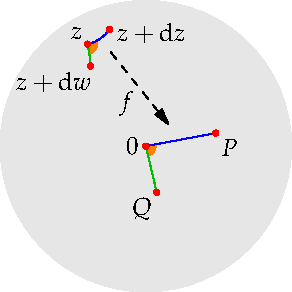
\includegraphics{isom-arclength}
\end{minipage}\par
where we deleted the $\cl z\,\dz$ term since it is infinitesimally small compared to $1-\nm z^2$.\smallbreak
Since isometries must preserve length and angle, this construction has several consequences:
\begin{description}
	\item[Angle measure]\phantomsection\label{pg:hypareaext} If we repeat the exercise for a second infinitesimal \textcolor{Green}{segment} $z\to z+\dw$, we see that the \textcolor{orange}{angle} between the original segments is precisely that between the infinitesimal vectors $\dz$ and $\dw$. This is precisely the conformality observation in Theorem \ref{thm:mobius}, and moreover shows how the distance function determines the angle measure.
	\item[Infinitesimal distance and arc-length] The hyperbolic distance from $z$ to $z+\dz$ is
	\[d(z,z+\dz)=d(O,P)=\ln\frac{1+\nm P}{1-\nm P} =\ln(1+\nm{P})-\ln(1-\nm{P})=2\nm{P}=\frac{2\nm{\dz}}{1-\nm{z(t)}^2}\]
	where the approximation $\ln(1\pm\nm P)=\pm\nm P$ is used since $\nm P$ is infinitesimal.\smallbreak
	If $z(t)$ parametrizes a curve in the disk, then the infinitesimal distance formula allows us to compute the arc-length
	\[\int_{t_0}^{t_1}\frac{2\nm{z'(t)}}{1-\nm{z(t)}^2}\,\dt\]
	\item[Area] If $\dx$ and $i\dy$ are infinitesimal horizontal and vertical changes in $z=x+iy$, then the area of the infinitesimal rectangle spanned by $z\to z+\dx$ and $z\to z+i\dy$ is the area element
	\[\dA=\frac{2\,\dx}{1-\nm z^2}\frac{2\,\dy}{1-\nm z^2} =\frac{4\,\dx\dy}{(1-x^2-y^2)^2}\]
	The area of a region $R$ in the Poincaré disk is therefore given by the double integrals
	\[\iint_R\frac{4\,\dx\dy}{(1-x^2-y^2)^2}=\iint_R\frac{4r\,\dr\,\dth}{(1-r^2)^2} =\iint_R\sinh\delta\,\D\delta\,\dth\]
	where the last expression is written in polar co-ordinates using the hyperbolic distance $\delta$. In this way the measure of area also depends on the distance function.
\end{description}

\begin{example}{Circles and `hyperbolic $\pi$'}{}
Suppose that a circle has hyperbolic radius $\delta$. By moving its center to the origin via an isometry, we can parametrize it in the usual manner:
\[z(t)=r\twovec{\cos\theta}{\sin\theta},\quad \theta\in[0,2\pi)\quad\text{where}\quad \delta=\ln\frac{1+r}{1-r}\rightsquigarrow r=\frac{e^\delta-1}{e^\delta+1}\]
Its circumference (hyperbolic arc-length) is then
\[\int_0^{2\pi}\frac{2 r}{1-r^2}\,\dth=\frac{4\pi r}{1-r^2}=2\pi\sinh\delta=2\pi\left(\delta+\frac{1}{3!}\delta^3+\frac{1}{4!}\delta^5+\cdots\right)>2\pi\delta\]
where we used the Maclaurin series to compare. Its area is
\[\int_0^{2\pi}\int_0^\delta\sinh\delta\,\D\delta\,\dth =2\pi(\cosh\delta-1)=\pi\left(\delta^2+\frac{2}{4!}\delta^4+\frac{2}{6!}\delta^6+\cdots\right)>\pi\delta^2\]
A hyperbolic circle therefore has larger ratios of circumference\,:\,radius and area\,:\,radius${}^2$ than for a Euclidean circle. Moreover, these ratios are \emph{not constant}: one might say that the hyperbolic version of $\pi$ is a function!
\end{example}

\boldinline{Hyperbolic Lines as Geodesics}

Finally, we perform a calculus of variations argument to see that the distance function in fact \emph{defines} our notion of a hyperbolic line.

\begin{defn*}{}{}
A \emph{geodesic} is a path of shortest length between two points.
\end{defn*}

\begin{thm*}{}{}
The geodesics in the Poincaré disk model are precisely the hyperbolic lines.
\end{thm*}

\begin{proof}
First suppose that $b$ lies on the positive $x$-axis. Parametrize a curve from $0$ to $b$ via
\[z(t)=x(t)+iy(t)\quad\text{where}\quad 0\le t\le 1,\quad z(0)=0,\ z(1)=b\]
Now compute its arc-length:
\begin{align*}
\int_{0}^{1}\frac{2\nm{z'(t)}}{1-\nm{z(t)}^2}\,\dt&=\int_{0}^{1}\frac{2\sqrt{x'^2+y'^2}}{1-x^2-y^2}\,\dt\ge \int_{0}^{1}\frac{2\nm{x'}}{1-x^2}\,\dt\ge \int_{0}^{1}\frac{2x'(t)}{1-x(t)^2}\,\dt =\int_0^b\frac{2\,\dx}{1-x^2}\\
& =\ln\frac{1+b}{1-b}=d(0,b)
\end{align*}
where we have equality if and only if $y(t)\equiv 0$ and $x(t)$ is increasing. The length-minimizing path is therefore along the $x$-axis.\smallbreak
More generally, given points $A,B$, apply an isometry $f$ such that $f(A)=0$ and $f(B)=b$ lies on the positive $x$-axis. The geodesic from $A$ to $B$ is therefore the image of the segment $\cl{0b}$ under the inverse isometry $f^{-1}$. By the properties of Möbius transforms, this is an arc of a Euclidean circle through $A,B$ intersecting the unit circle at right-angles: our original definition of a hyperbolic line.
\end{proof}
